\chapter{Resolving a Conducting Conformation of CFTR Using Free Energy Calculations}
\label{chap:opening}
\chapquote{You wanna fight?} {- Doctor Zachary Picker. Layperson. (personal communication)}
\setcounter{figure}{0}
\renewcommand{\thefigure}{\arabic{chapter}.\arabic{figure}}


\section*{\centering Abstract} 
The misfunction of the CFTR gene causes Cystic Fibrosis. This protein conducts both chloride and bicarbonate. Recent advances have demonstrated the power in potentiating the conductance of CFTR to relieve disease symptoms. Hence, determining the precise mechanism behind ion conduction has important implications for ongoing drug discovery efforts. 

Existing atomic structures of CFTR raise unresolved questions as to how CFTR conducts ions, as they exhibit a constriction smaller than the ions themselves. This indicates that there must be some conformational changes for ions to pass through CFTR. Here we present innovative simulation techniques combining unbiased molecular dynamics principal component analysis, OPES-Metadynamics and umbrella sampling to resolve the conduction pathway through the selectivity filter of human CFTR. We also propose electrophysiology experiments to experimentally test whether this conformation is physiologically important.  

The findings of this study demonstrate that computational power and protein forcefields are now sufficiently developed to take the advances of the era of structural abundance brought about by the cryo-EM ``resolution revolution" and AI based protein structure predictions, to elucidate even more of the protein conformational landscape. This heralds an exciting new era of computational structural biology and biophysics.


\section{Introduction}

Ion channels are crucial clinical to many cellular functions. They are pursued for many clinical reasons, such as the treatment of disease and the relief of pain \cite{}. The mechanism and conditions under which they open and close is a closely studied topic due to the ability of small molecule drugs to regulate this transition and the pathology that a dysfunctional channel can cause, either from mutation or environmental changes.

One of the most well-known channelopathies is the misfunction of the anion channel, the Cystic Fibrosis Transmembrane conductance Regulator (CFTR) which causes Cystic Fibrosis (CF) \cite{riordan1989,gadsby2006}. This is a fatal genetic condition which afflicts an estimated 162000 people worldwide, with a significant population unable to access treatment \cite{guo2022}.

Various mutations may cause this ion channel to misfunction but the discovery of new small molecules known as modulators heralds a new era in the treatment of this life-limiting disease \cite{}. There are two classes of these modulators, correctors which assist the protein to fold into the right shape, and potentiators which facilitate the proteins transition from the closed to the open, conducting state. 

Due to the importance of the conductance of this channel in disease pathology, a molecular understanding behind the basis of its conductivity will inform the rational design of novel therapeutics to improve patient outcomes. Unfortunately, current available structures of CFTR are insufficiently dilated in order to conduct anions \cite{}. MD simulations with a strong applied electric field were able to observe the permeation of chloride ions through the channel \cite{}. However, the number of conduction events these authors observed would imply a conductivity of X pS (17 events in 10 $\mu$s of sampling) . this conduction rate is rate an order of magnitude below the experimentally measured conductivity of the CFTR (). Metadynamics of the zebrafish CFTR structure were also able to resolve a conduction pathway for chloride ions, but these calculations also exhibited a significant free energy barrier to the  passage of chloride (X kcal/mol). These two studies indicate that there are likely conformational states not yet experimentally visualised which will support the conduction of chloride. 

We note also, that previous MD studies have focussed on the conduction of chloride, since it is the most physiologically important species to permeate through CFTR. However, larger ions such as bicarbonate and glutathione have also been shown to move through CFTR and play an important role in the pathogenesis of disease \cite{}. Hence, it is clear that there is a need to move beyond the available cryo-EM structures of CFTR to resolve the conducting conformation. Here we present \textit{in silico} methods to compliment this existing structural information. 

The conduction pathway of CFTR can be split into two sections. The inner vestibule and the selectivity filter. We have previously studied conduction through the inner vestibule in chapter \ref{chap:R352Q} \cite{wong2022a}, and in this chapter we will study the conduction through the selectivity filter. 

In CFTR, the selectivity filter is thought to be narrow, as mutations which reduce the volume of pore lining amino acids lead to a loss of selectivity, for example F337A and to a lesser extent L102A \cite{}. However, the pore is likely not as narrow as those found in potassium channels, as CFTR is only weakly selective \cite{}. 

Additionally, the sequence of permeatbility of annions is correlated by their lyotropic, indicating that partial dehydration of the annions is likely during their passage through the selectivity filter. Despite these characteristics, CFTR is only weakly selective, permeating a large set of annions such as chloride, bicarbonate and glutathione \cite{}. We will investigate the permeation of the former two in this chapter. 

Resolving the conduction mechanism of ion channels has bene of keen interests to the computational biophysics community for some time, as this mechanism is responsible for regulating many cellular processes \cite{black2020}. To my knowledge, this one of the first studies which has been able to take a non-conducting conformation of an ion channel and then dilate it in order to understand the full conduction pathway. 

A similar technique could be used in many ion channels which have been imaged very close to their active conformation but during the imaging process they change conformation slightly. Hence, the techniques employed in this chapter could be applied to other important protein systems such as P-glycoprotein \cite{}.  %make sure you cite more things.

A recent, careful, electrophysiology study into the kinetics of the R117H mutation has given important implications for the work presented here \cite{}. Before this study it was thought that R117 forms a salt bridge with E1126 \cite{cui2014}. But in fact, the experiments in the former publication found that it is E1124 which makes a connection to R117, by interacting with the carboxyl oxygen atom in the backbone of R117, not E1126. This situation leaves the role of E1126 in channel gating kinetics unknown, but through our \textit{in silico} experiments, we will show how in the open of CFTR, E1126 forms a salt bridge with R334. This may be tested through single ion channel electrophysiology experiments.

The work presented in this chapter differs in an important way from existing computational studies. Many previous attempts to induce conformational changes have usually been \textit{targetted}, that is, they have usually sought to resolve the energy landscape \textit{between} experimentally determined structural conformations the protein, or a closely related one \cite{, lev2020, bergh2021, mccomas2022}. Since there is not yet an experimentally determined atomistic structure of CFTR, the presented study is instead \textit{untargetted}. Hence, by combining subtle hints from \textit{in vitro} biophysical experiments on CFTR with results from our unbiased MD simulations, we chose collective variables which might let us resolve a conducting conformation of CFTR. This signals how computational methods have become sufficiently developed to use experimentally obtained structural snapshots as starting points to explore the local neighbourhood. This approach has the potential to discover new drug binding pockets and novel molecular mechanisms within cells \cite{}.

\section{Results}

\subsection{Long Simulations Reveal Motions which Dilate the Pore of CFTR}
Four independent replicates unbiased MD were run for the WT-CFTR system. These were run for at least 2 microseconds each, for a combined total of 8.2 $\mu$s of simulation time. 

In post processing, the motions of the transmembrane helices were analysed using Principal Component Analysis \cite{pearson1901, hotelling1936}. This revealed large motions in TMs1 and 6 in directions which dilated the extracellular pore (Figure \ref{PCA_motions}).  

\begin{figure}
	\begin{center}
		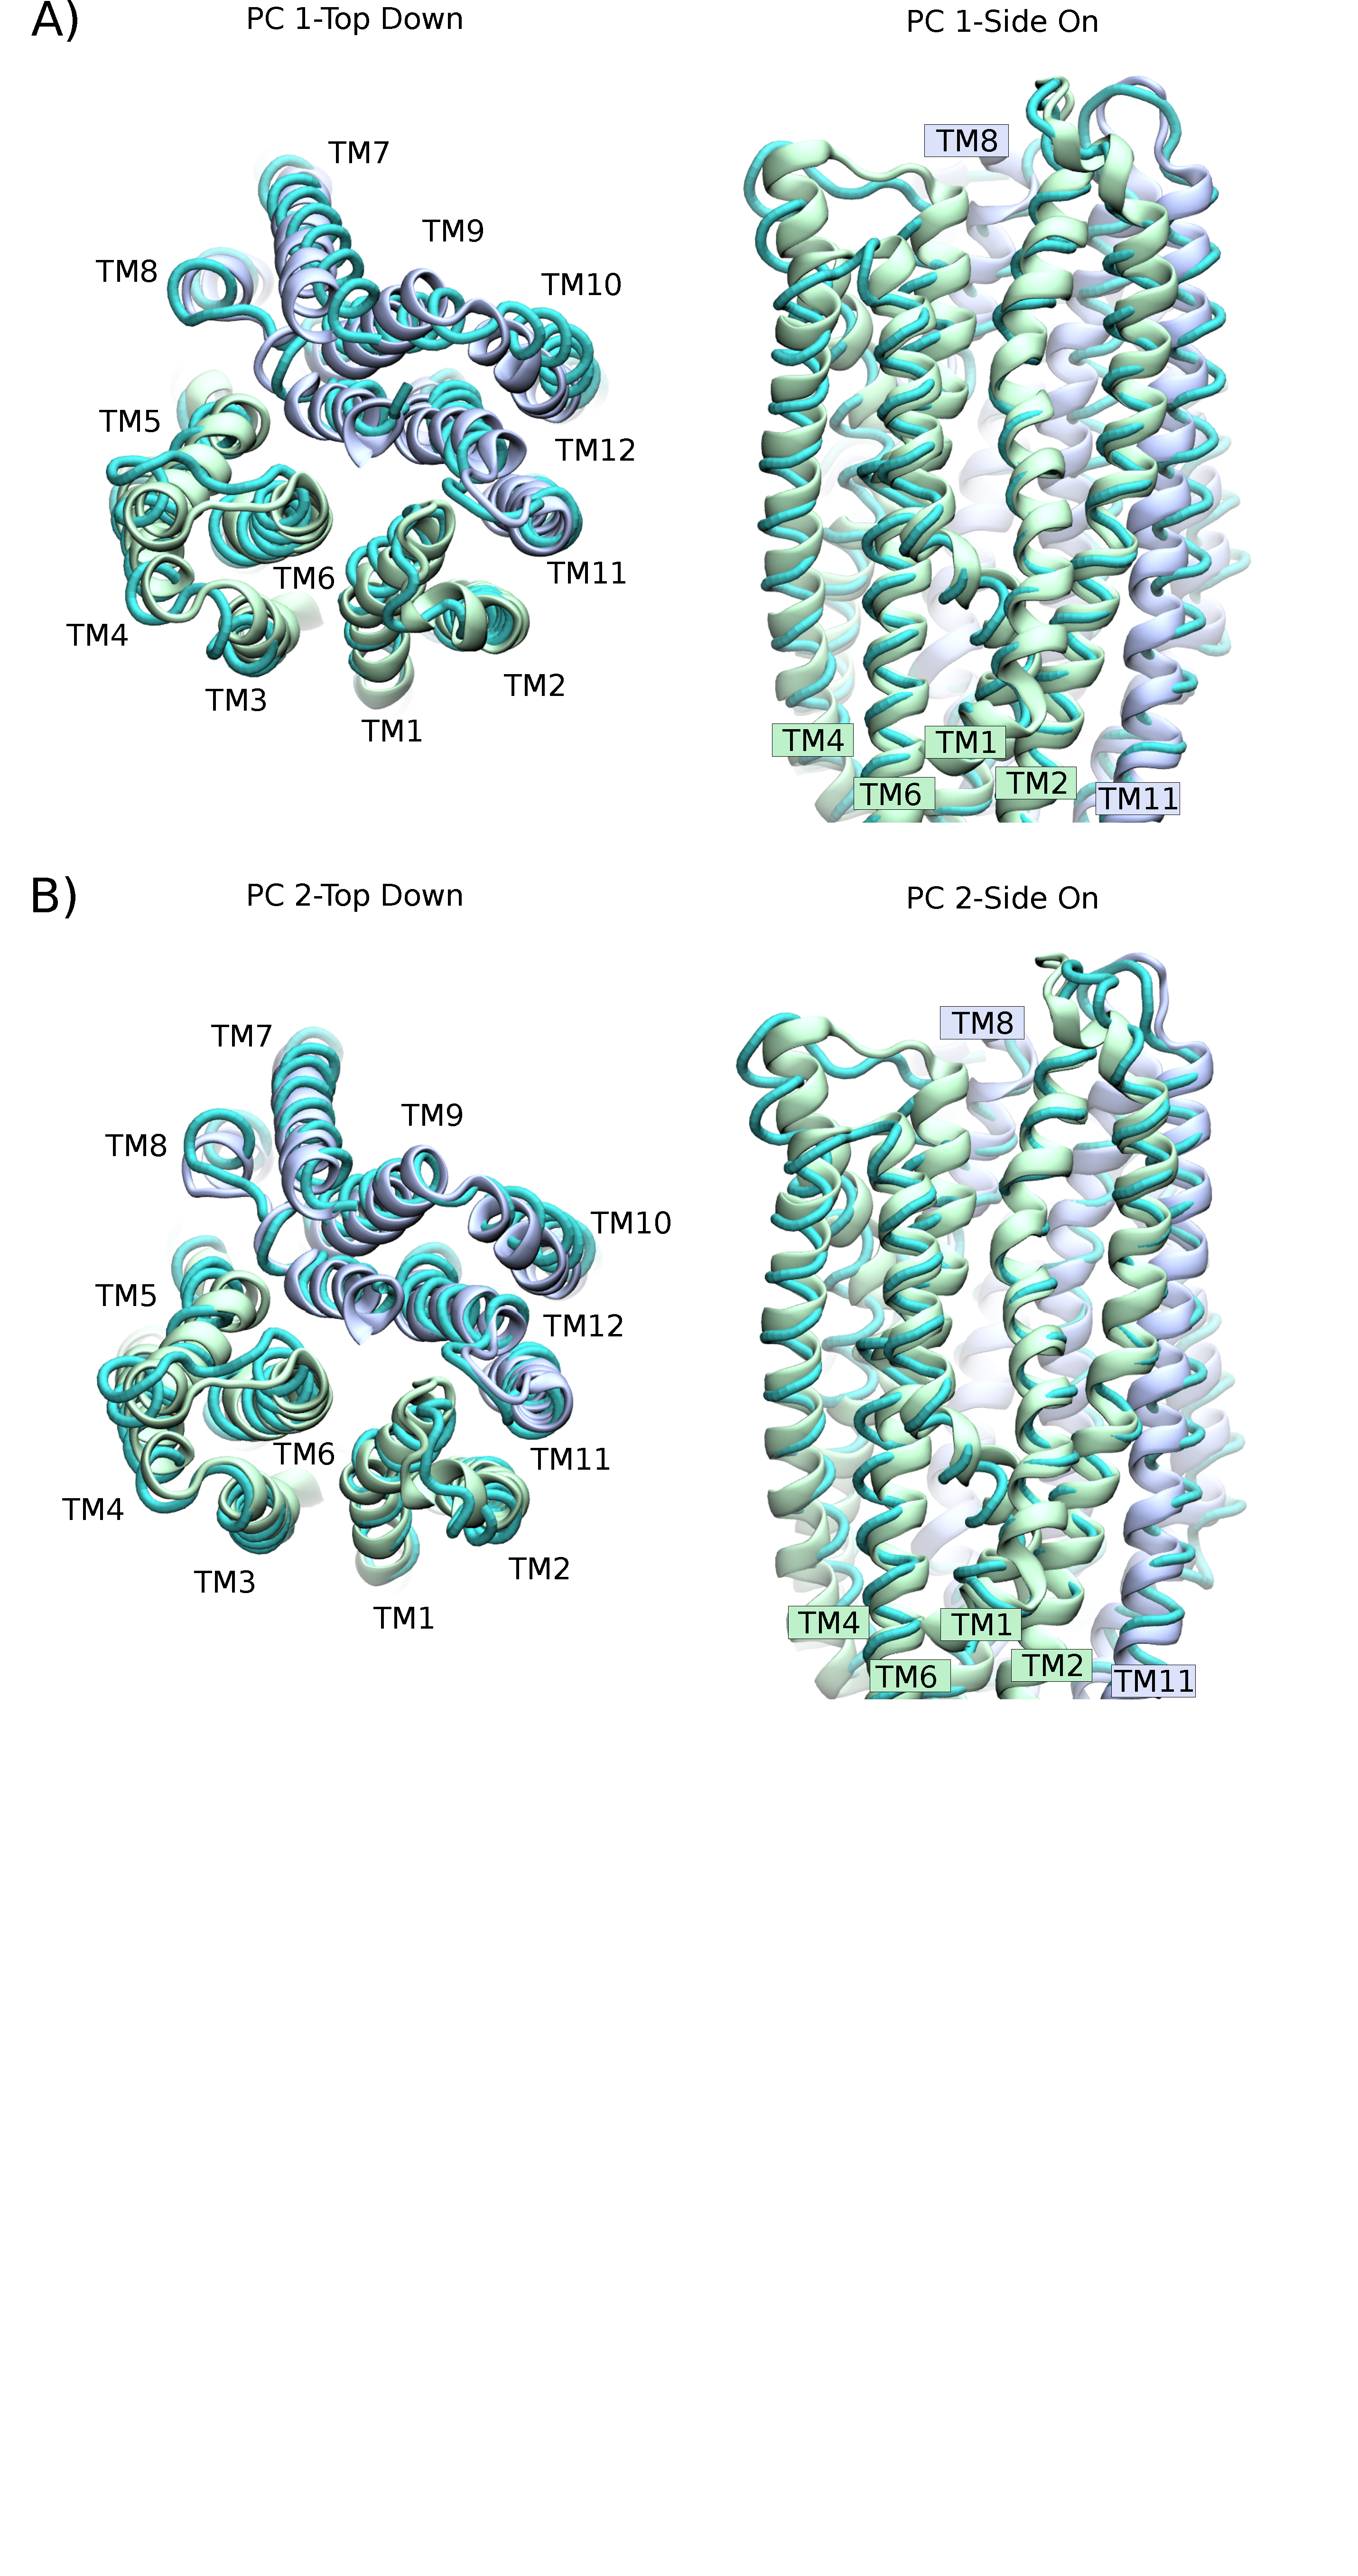
\includegraphics[width=1\textwidth]{figures/opening/pca_motions.pdf}
	\end{center}
	\captionsetup{singlelinecheck = false, justification=raggedright}
	\caption[Principal Component Analysis Reveals Large Motions in CFTR Transmembrane Helices] {\textbf{Principal Component Analysis Reveals Large Motions in CFTR Transmembrane Helices}}{A) Visualisation of the results from principal component analysis from 4 independent simulations, comprising 8.2 $\mu s$ of unbiased MD sampling. Motions along the first two principal component vectors were found to capture 38\% of the variation in the simulation and were used in further analysis. B) Visualisation of the first principal component vector (PC1). Note the motion in TMs 1, 6 and 8 C) Visualisation of the second principal component vector (PC2). Note the motions in TMs 1 and 6 but in directions orthogonal to PC1. D) Visualiastion of the Dilated Open state which we will analyse in detail in subsequent sections. This structure was obtained by a linear combination of PC 1 and 2 followed by unbiased MD simulation.} 
	\label{PCA_motions}
\end{figure}

Choosing CVs from these unbiased statistics is not trivial. We found that the first two Principal Components represented 38\% of the kinetic variance in the unbiased data. Additionally, they appeared to cpature motions in TM1 and TM6, which is where we expected the dilation to occur, given the experimentally determined location of the selectivity filter \cite{linsdell2018, negoda2018, negoda2019}. A more detailed discussion of our choice in CVs can be found in section \ref{supp_cv_choice} and are visualised in \ref{CV_choice_figb}. 

The amino acids chosen for Principal Component Analysis were chosen carefully (Table \ref{motions_table}). Amino acids in disordered loops were excluded from analysis as they make large motions quickly. These large, fast motions would distort the optimal, slow degrees of freedom which we would hope to investigate with free energy calculations \cite{noe2001}. 

Since the more atoms included in our collective variables the slower our calculations would run, we limited subsequent free energy calculations to a set the helices directly surrounding the pore. This is shown in Figure \ref{}, this was the same technique employed in \cite{hoffman2018}.

\subsection{OPES-Metadynamics Finds a Stable Conformation with an Open Extracellular Pore}

The principal components derived in the previous section were used as collective variables to study the motion of the pore lining transmembrane helices. A two dimensional Free Energy Surface along these CVs was constructed through the use of 8 independent walkers, each running for $1.5\mu$s with OPES metadynamics with a barrier parameter of 38.2 kcal/mol. The resultant surface can be seen in Figure \ref{summary_FES}A, and convergence of this FES is demonstrated in \ref{convergence_FES}. 

Note the presence of a local free energy minima at (0.10, 0.21) in Figure \ref{summary_FES}A. When this coordinate in CV space was investigated with unbiased MD, we noticed that the extracellular pore had dilated significantly (Figure \ref{summary_FES}B). Further, we found that the dilated configuration was stable on time-scales up to 500ns, with the constriction  was found that the protein remained in a conformation which dilated the pore to almost 3 $\AA$. This larger opening was in the right place between TM1 and TM6 and of a size which we would expect for anions known to pass through CFTR. 

This completely removed the aberant constriction from the cryo-EM structure of CFTR (Figure \ref{summary_FES}D). This 

\begin{figure}
	\begin{center}
		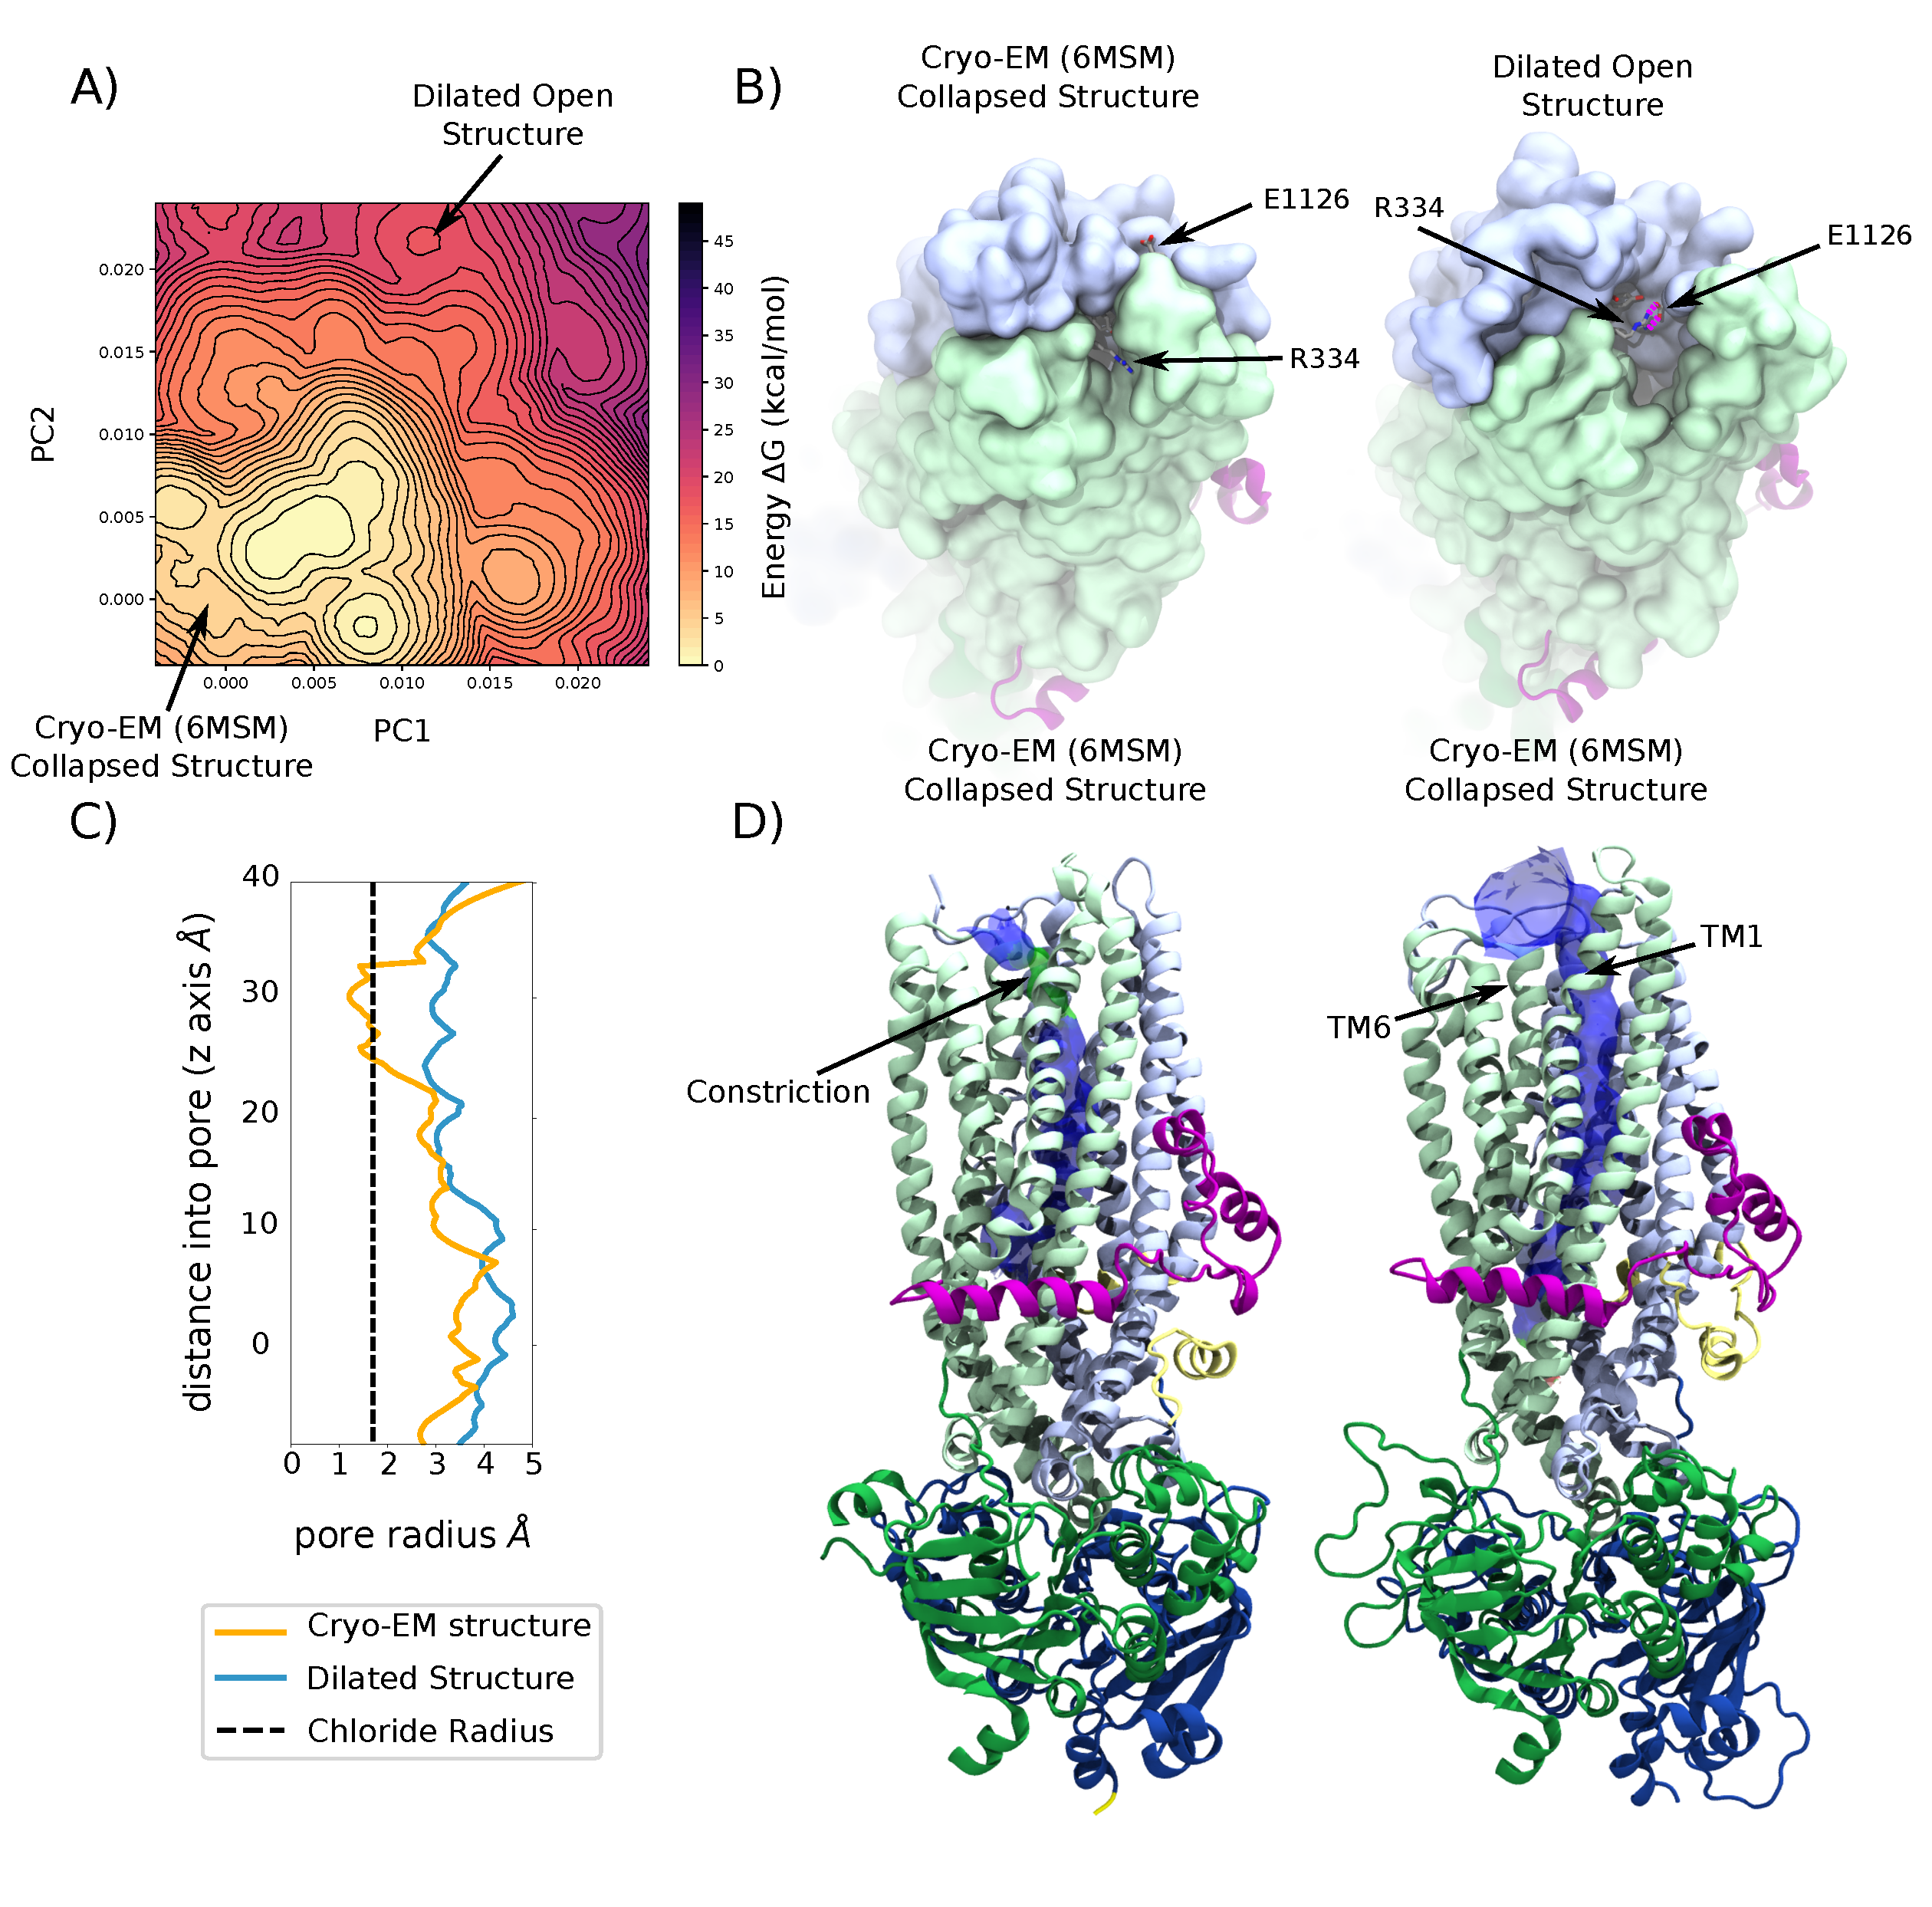
\includegraphics[width=1\textwidth]{figures/opening/summary_dilated_structure_1.pdf}
	\end{center}
	\captionsetup{singlelinecheck = false, justification=raggedright}
	\caption[Free Energy Calculations Discover a Dilated, Conformation of CFTR.] {\textbf{Free Energy Calculations Discover a Dilated, Conformation of CFTR.}}{A) The free energy landscape obtained along PC 1 and 2 through OPES-Metadynamics. Note the free energy minimum corresponding to a collapsed structure, found cryogenic electron micrcoscopy in the bottom left and the free energy minimum at (0.01,0.021). This latter well was found to correspond to a stable, structure which appears capable of passing anions. B) A visual comparison between the constricted structure and our dilated open strcuture. Note how the extracellaulr opening is much wider in the dilated strcuture. The R334 and E1126 amino acids are visualised to show how they come into contact with eachother in the dilated structure. C) A quantiative measuremnt of the pore radius for different conformations of CFTR, generated with HOLE2 \cite{smart1996}. Dehydrated chloride has a radius of 1.7 $\AA$, while the collapsed cryo-EM structure of hCFTR exhibits a constriction of 1.2 $\AA$, so even if chloride were to be dehydrated during its migration through the selectivity filter, there would need to be some change to the protein conformation. By contrast, the dilated open structure exhibits a constriction of 2.8 $\AA$ at its  narrowest point. This would be large enough to support the conduction of a diverse set of anions.  D) A side on comparison between the collapsed cryo-EM structure and the dilated open structure. The green constriction denotes the region too small to pass ions. This constriction has been completed removed in the dilated open structure we will study. }
	\label{summary_FES}
\end{figure}


\subsection{This open conformation gives rise to a novel salt bridge}
\label{salt_bridge}
The Free energy surface in figure \ref{summary_FES}A demonstrates molecular contributions which might stabilise this open configuration. It was possible that the dilatied structure was stabilised by simple hydrophylic interactions, as previous work has shown that the pore can wet and de-wet \cite{}, but we were curious if there were some novel protien-protein interactions which might be contributing to the discovered stable strcuture. 

In order to look for molecular interactions which might stabilise this open conformation, we inspected the interactions between pairs of positive and negative amino acids. It was found that a link between R334 and  E1126 could form in this new open state but not in the cryo-EM structure (Figure \ref{salt_bridge_fig}). This was possible due to the motions of TM6 and TM1, allowing E1126 on ECL5 to come closer to TM6. We expect this new salt bridge to be an important determining factor in stabilising the conducting conformation of CFTR.  

This is a novel interaction, where traces casn be found in the literature but not defninitilvey so given the important role of R334 in ion conductivity and gating. The implications of this will be outlined in the Discussion.

\begin{figure}
	\label{salt_bridge_fig}
	\begin{center}
		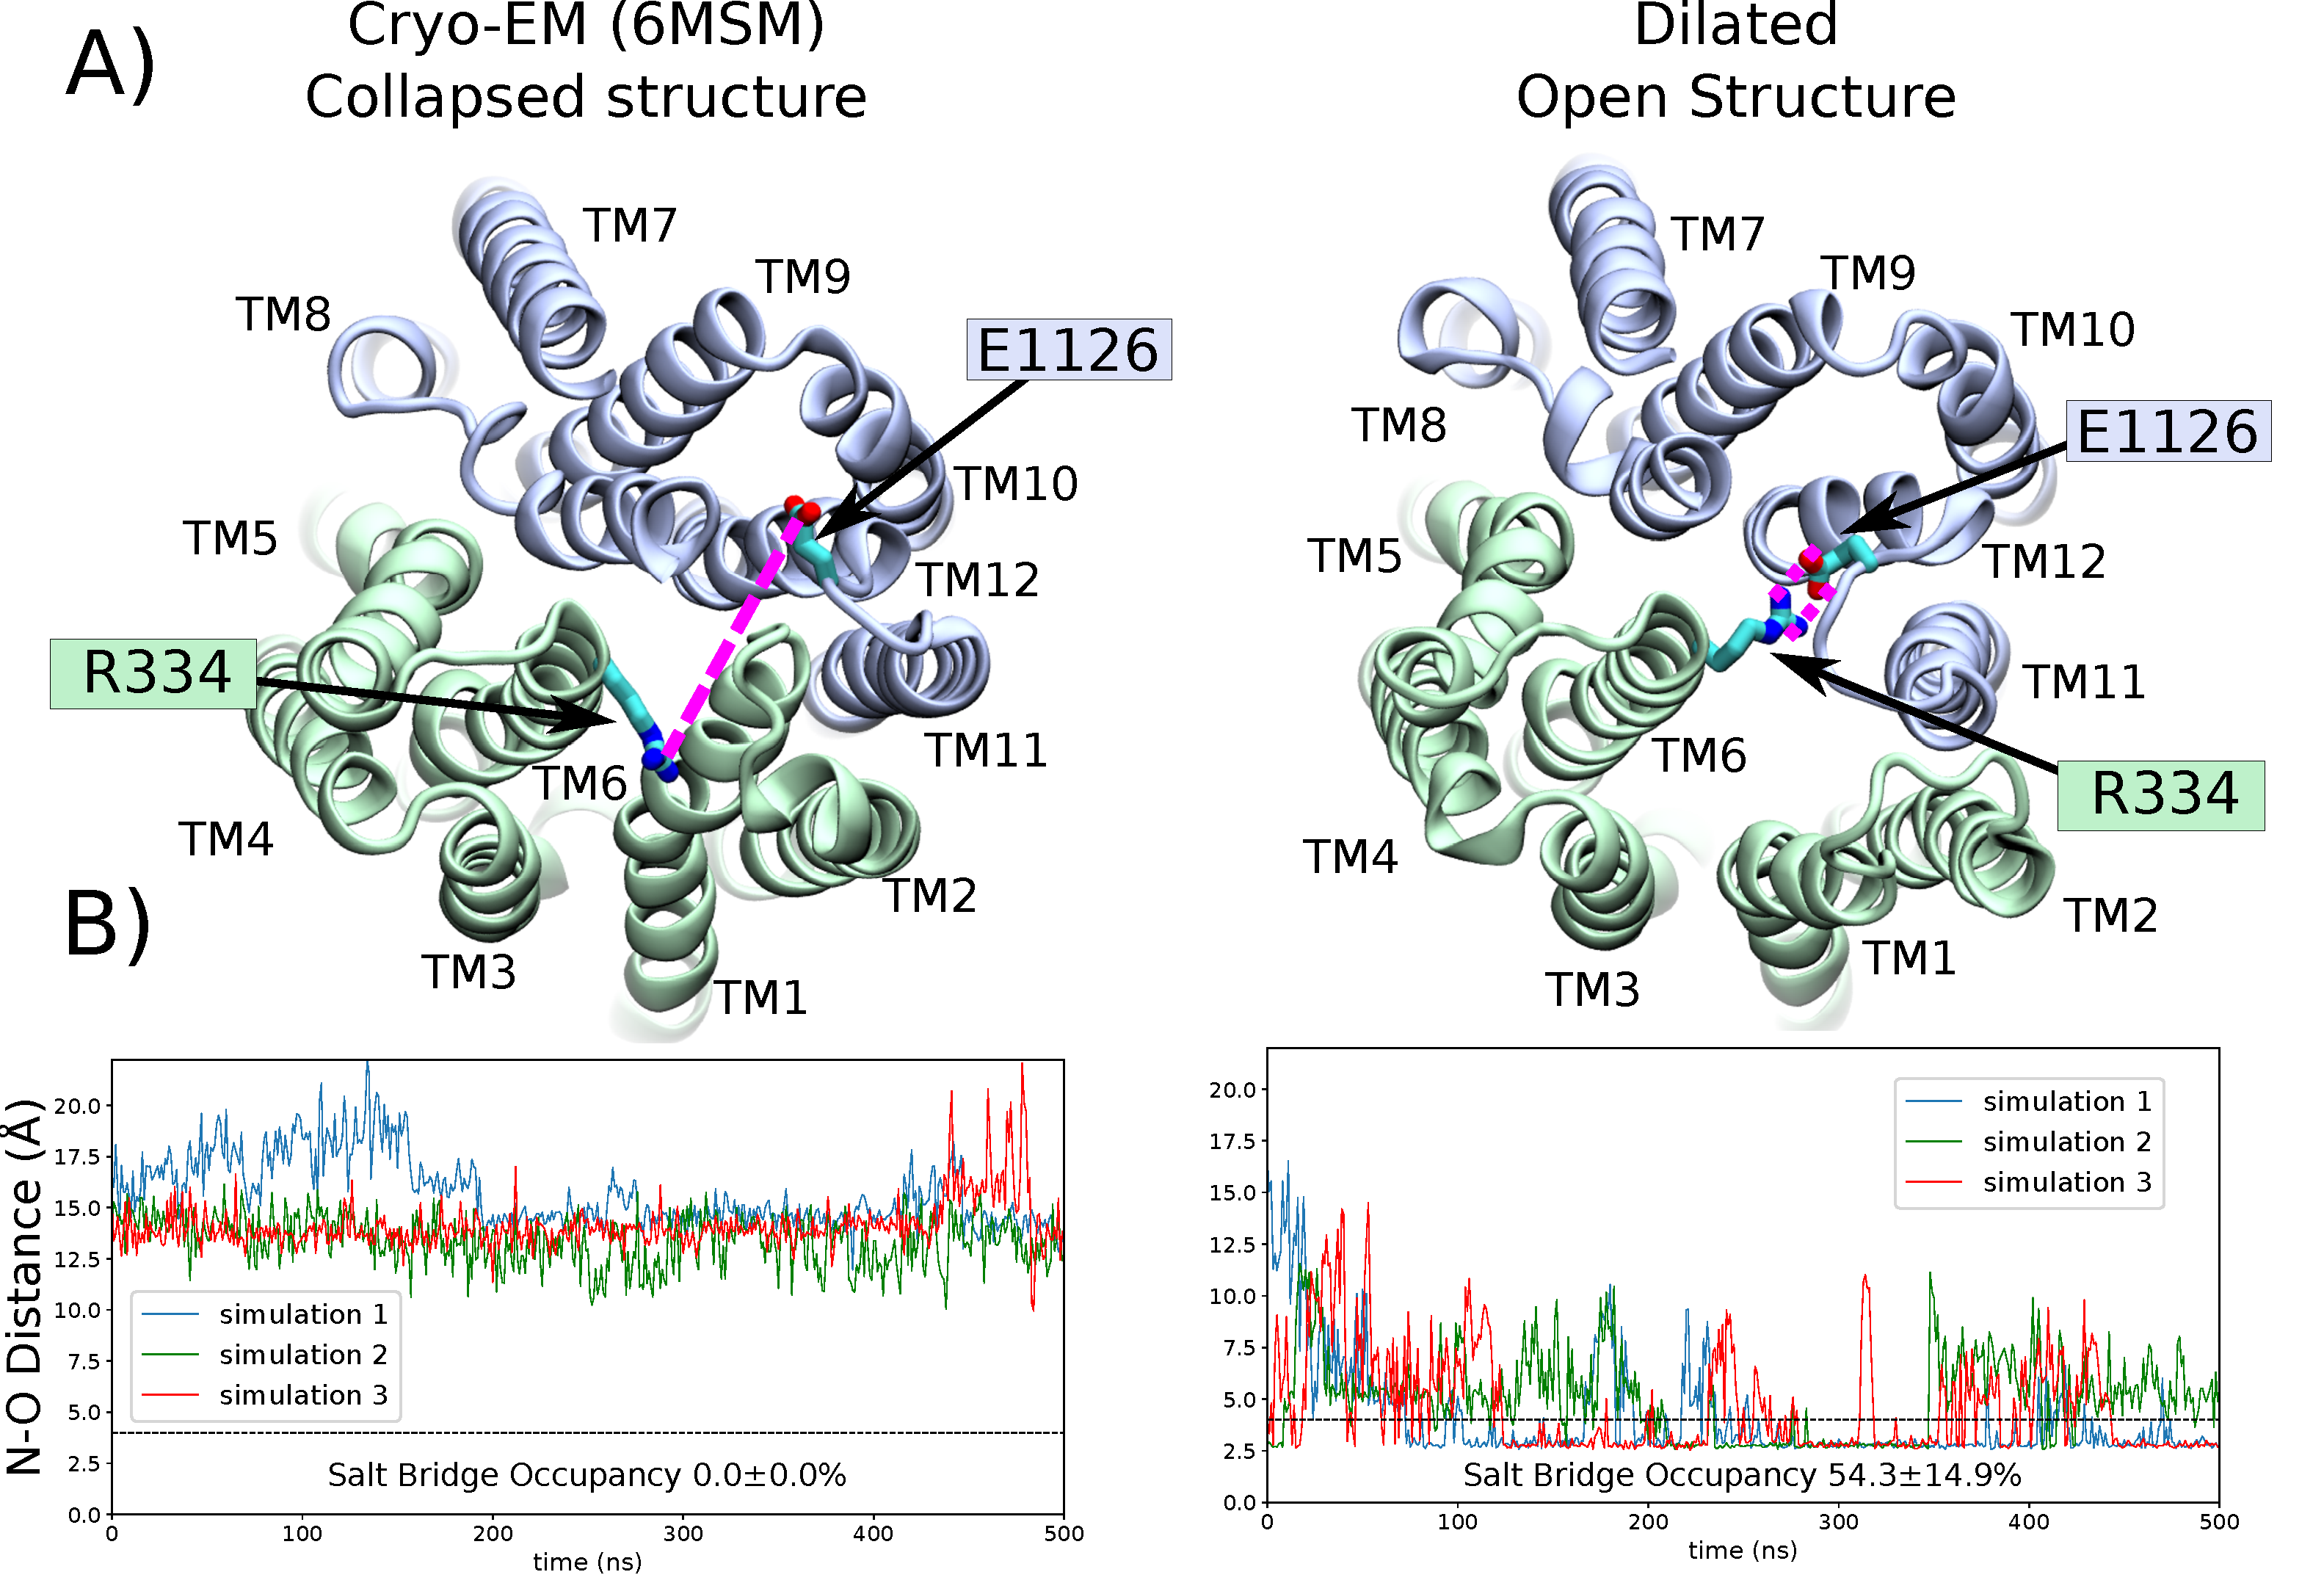
\includegraphics[width=1\textwidth]{figures/opening/salt_bridge_E1126_R334_figure.pdf}
	\end{center}
	\captionsetup{singlelinecheck = false, justification=raggedright}
	\caption[The Dilated Conformation of CFTR Gives Rise to the R334-E1126 Salt Bridge] {\textbf{The Dilated Conformation of CFTR Gives Rise to the R334-E1126 Salt Bridge}}{A) B) }
\end{figure}

\subsection{Proving the Open Conformation is capable of ion conduction with Umbrella Sampling}

In order to test the ability of the dilated structure to the conduct anions, we employed umbrella sampling. No restraints were placed on the configuration of the transmembrane helices during these free energy calculations. We constructed 4 PMFs this way, studying the conduction of chloride ions in the collapsed Cryo-EM structure, the dilated structure, and the dilated structure of R334W-CFTR. The latter 

The free energy landscape of ions through the selectivity filter in the cryo-EM structure is not amenable to the movement of ions. We obtained a sizeable barrier of 9.7kcal/mol to the passage of ions, demonstrating that without dilation this structure will not allow currents at a rate close to experimental measurements. By contrast, the dilated conformation which we discovered through metadynamics shows only a small free energy barrier of only 2.5 kcal/mol for both chloride and the larger bicarbonate. 

This small barrier roughly corresponds to what we would expect to be overcome by the natural 100mV polarisation of epithelial cells. Furthermore, the remarkably similar profiles for both bicarbonate and chloride are in agreement with the energy landscape we would expect from a weakly selective channel like CFTR. Indeed, the sampled landscape has calculated the pathway through the ``permeabilty selectivity filter" of CFTR, a region where we would expect the diffusion profile to differ between annions but not the . Deeper in the pore is the ''conductivity selectivity filter" which we might expect to display a difference between the two anions. The lower FES in the viccinity of K95 in Figure \ref{US_anions}C for bicarbonate compared to chloride may indicate tighter binding at this site, leading to lower conductnace. Unfortunately, there have not as many studies which have measured the effect of mutations on bicarbonate conductance but these results would lead us to epect that R134 and K95 play an important role in the permeation of this crucial molecular species. 

	\begin{center}
		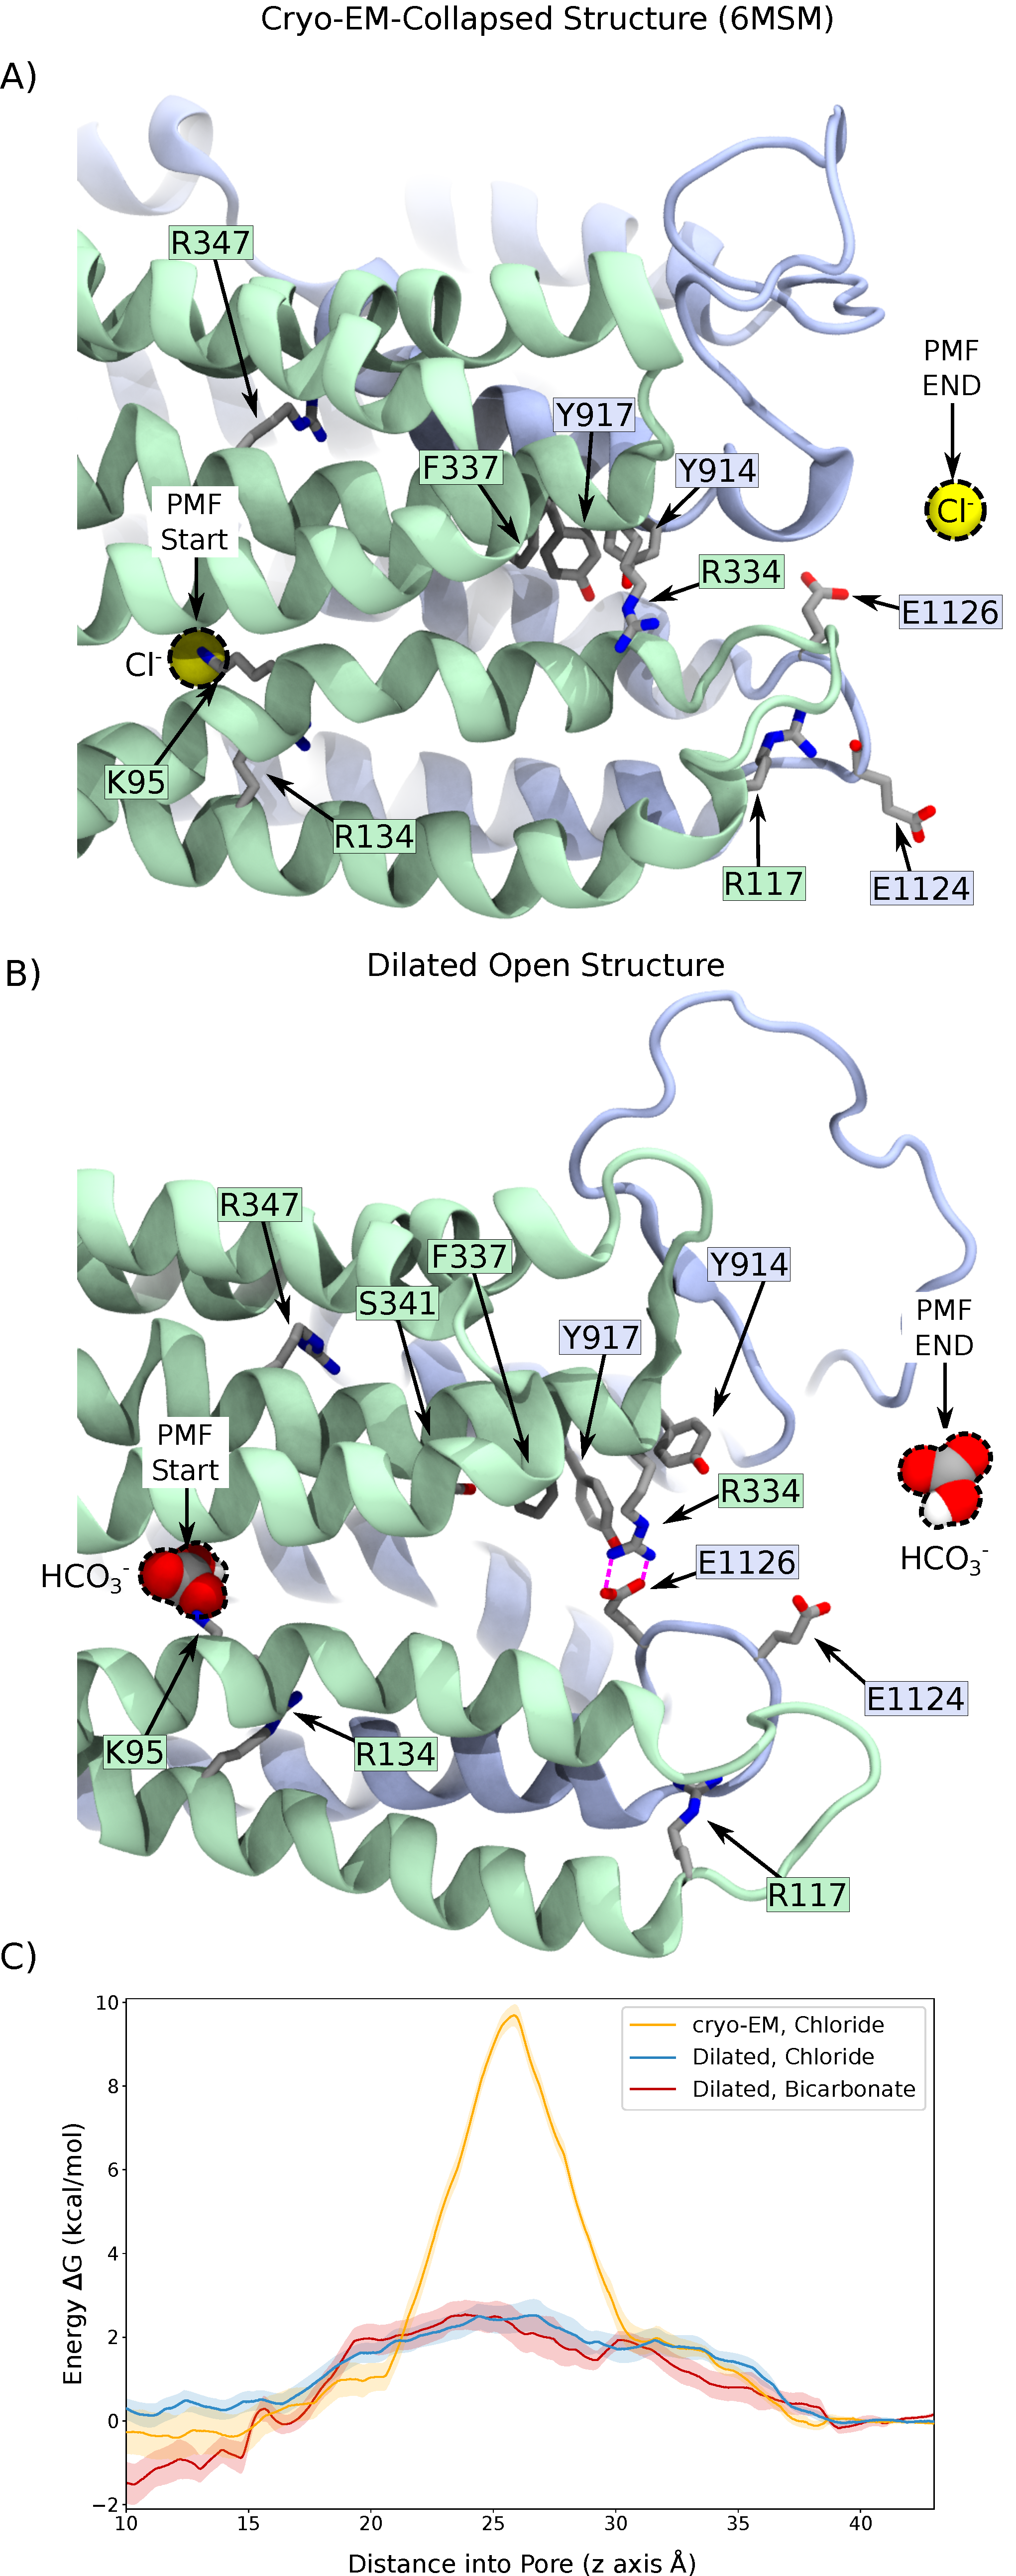
\includegraphics[width=0.6\textwidth]{figures/opening/pmf_fig_1_combined.pdf}
	\end{center}
\begingroup

	%\captionsetup{singlelinecheck = false, justification=raggedright}
	\captionof{figure}[The Dilated Conformation of CFTR is Capable of Conducting Anions] {\textbf{The Dilated Conformation of CFTR is Capable of Conducting Anions}}{A) A close-up visualisation of the selectivity filter in the collapsed cryo-EM structure. To pass through this structure the ion must move past a tight constriction formed by F337, Y914 and Y917. B) A visualisation of the selectivity filter in our dilated \textit{in silico} structure. Here, bicarbonate is pictured but the same structure was used to construct a PMF of chloride as well. The selectivity filter is not as constricted and R334 can make a salt bridge with E1126. This brings it closer to the conduction pathway where it can help coordinate the permeating anion. C) PMFs of the anions as they pass through the narrowest point in CFTRs permeation pathway. The collapsed cryo-EM structure exhibits a significant barrier to the conduction of chloride, this barrier is unphysically large and not what we expect given experimental measurements of this structure. By contrast, the dilated structure appears capable of permeating both chloride and bicarbonate, with a landscape in agreement with the characterisation of the channel found in experiments. }
	\label{US_anions}
	\endgroup



\subsection{This open state can be used to study disease causing mutations in the outer pore such as R334W}


\begin{figure}
	\label{R334_pmf}
	\begin{center}
		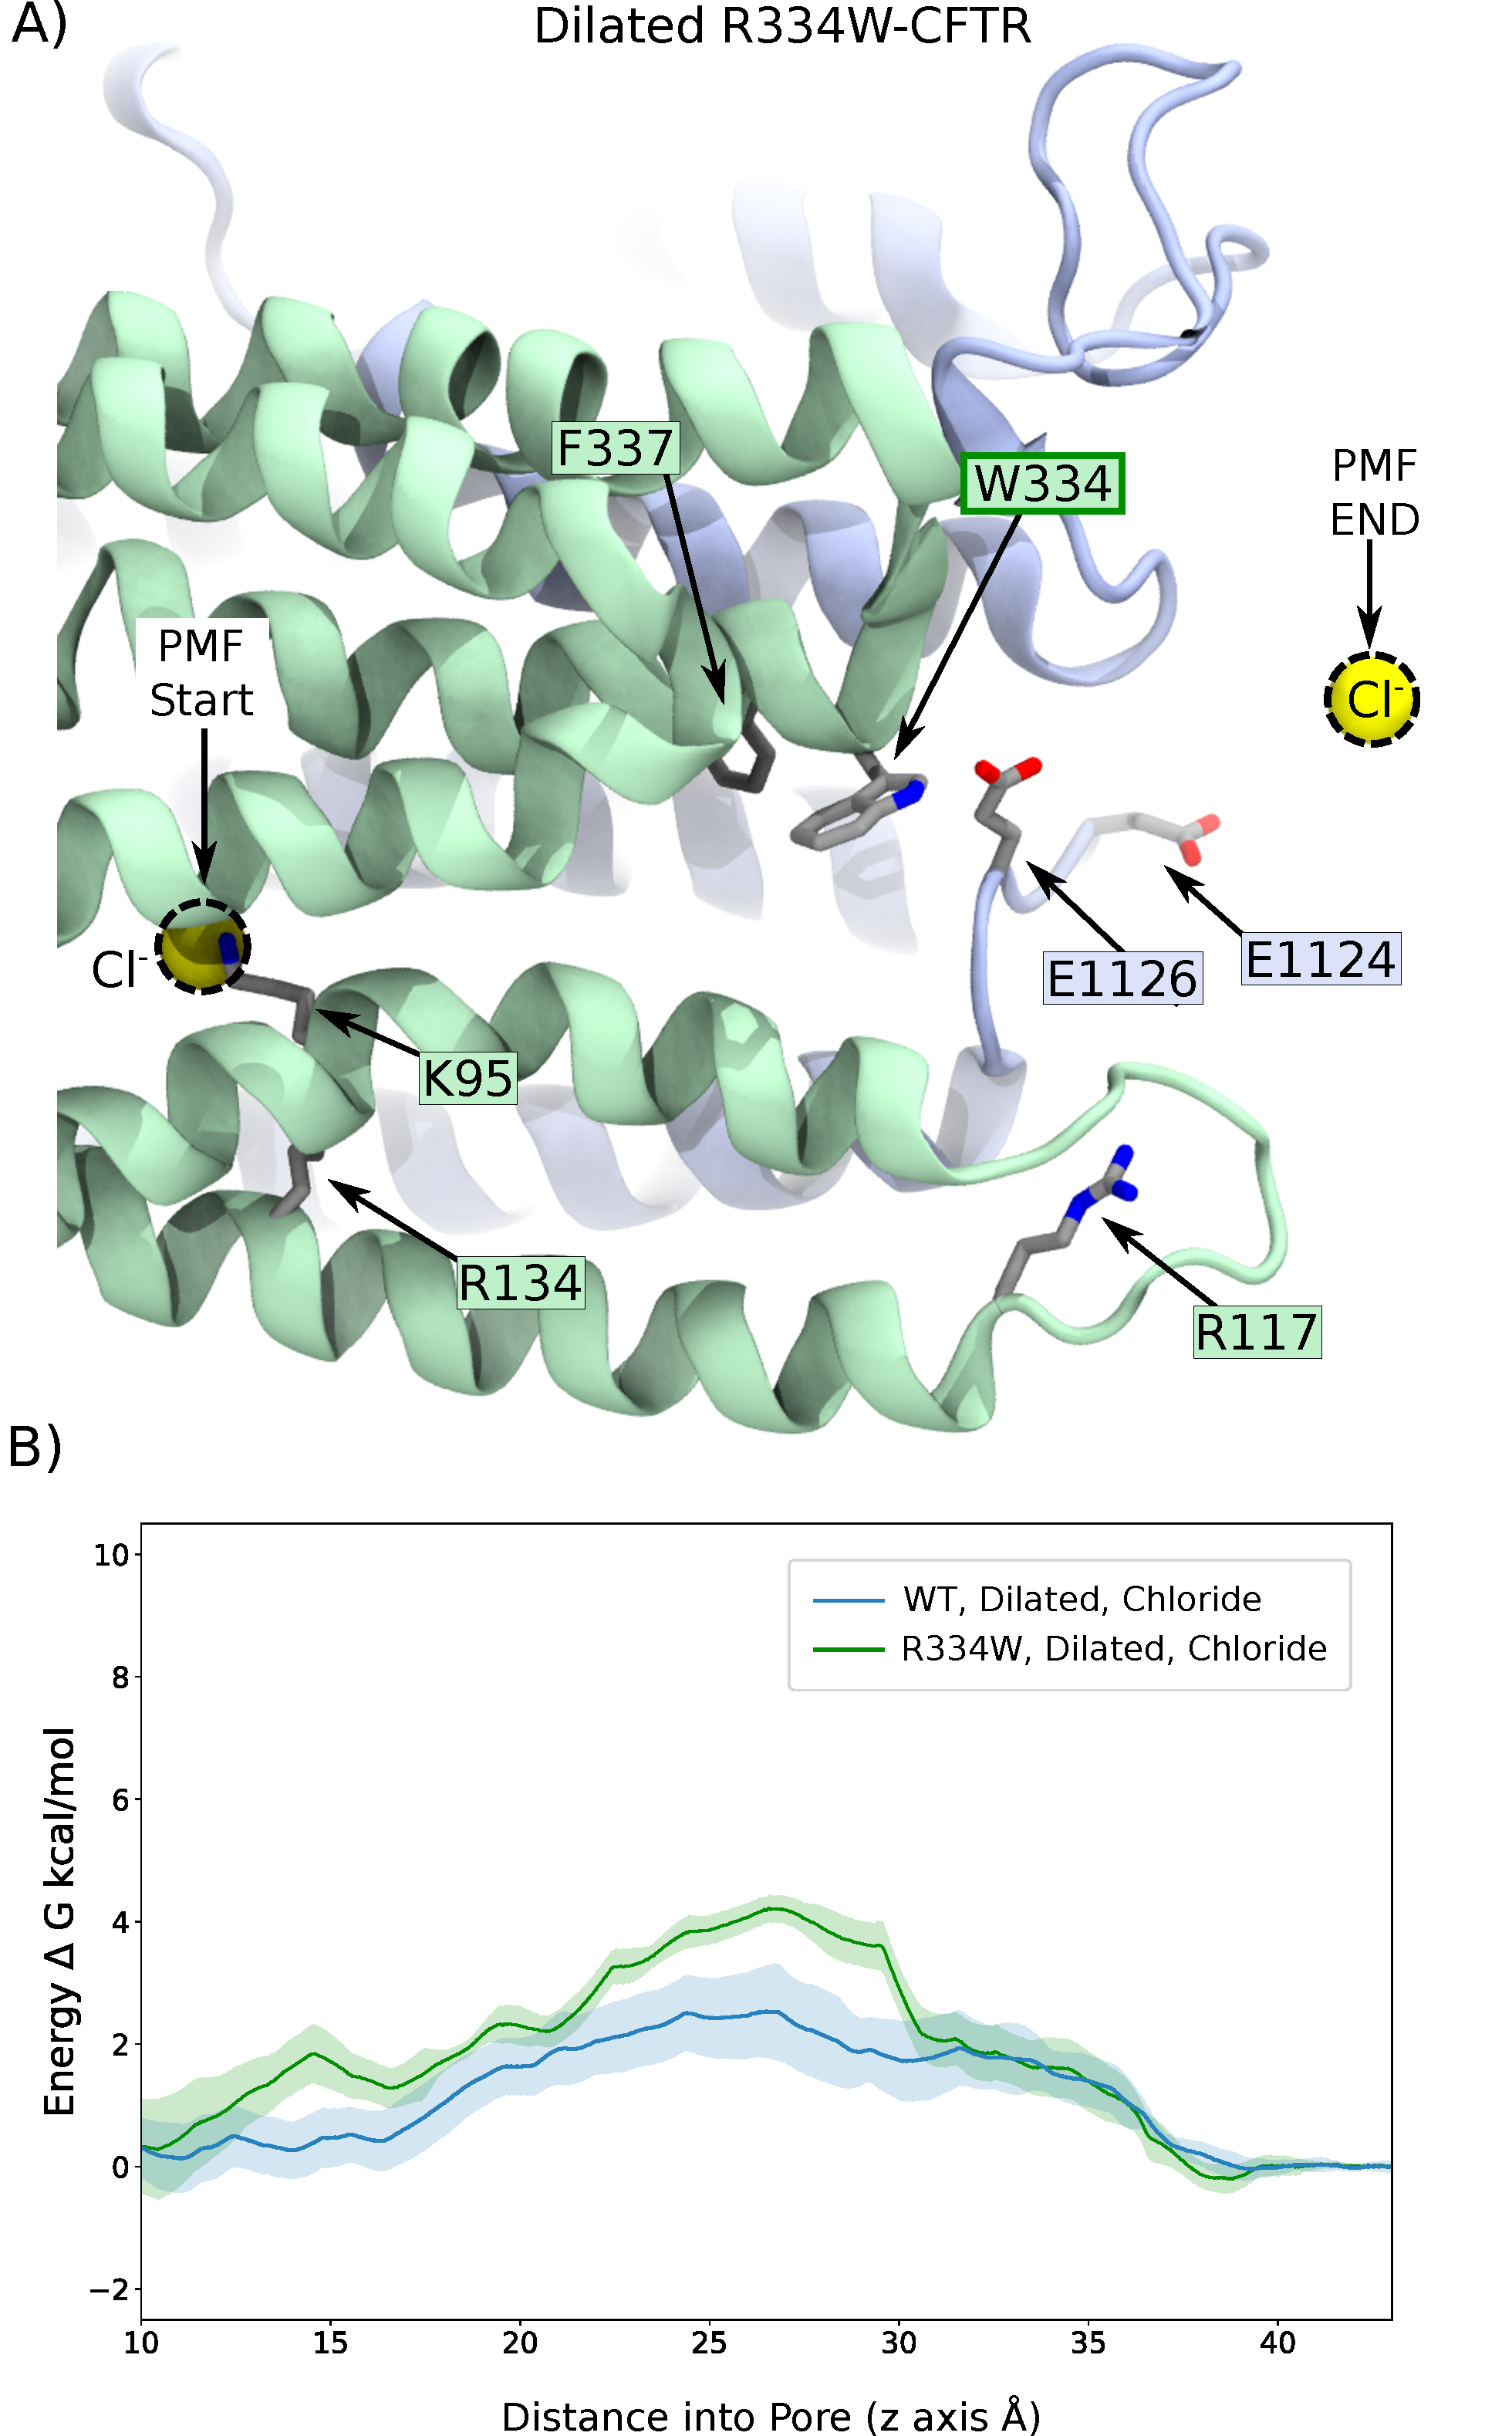
\includegraphics[width=0.6\textwidth]{figures/opening/R334W_pmf_combined.pdf}
	\end{center}
	\captionsetup{singlelinecheck = false, justification=raggedright}
	\caption[R334W Inhibits the Conduction of Anions] {\textbf{R334W inhibits the Conduction of Anions}}{A) A visualiation of R334W-CFTR in the dialted  conformation. Note how W334 is placed in the outer part of the pore. B) A PMF derived from Umbrella sampling to compare the energetics of the conductance of chloride through R334W-CFTR to WT-CFTR in the dilated conformation. The WT-CFTR curve has been reproduced from the same data in Figure \ref{US_anions}. The R334W-CFTR PMF exhibits a larger barrier compared to WT-CFTR indicating that the conduction of chloride will be inhibited in this mutation. It is likely that this 2.5 kcal/mol additional energy barrier has a paritucllarly deleterious effect on the conduction of the channel because it occurs at the narrowest part of the pore. There are no alternate pathways which might help compensate for the mutation, as was the case in R352Q in chapter \ref{chap:R352Q} \cite{wong2022a}.  }
\end{figure}

There are several disease causing CFTR mutations which occur at the extracellular mouth of the protein (E116K, R334[WQL],R117[HCP], I336K, S341P)\cite{cftr2}. Note how these are all clustered around TM1 and TM6. This is good evidence to suggest that this is the permeation pathway for chloride in hCFTR, as was found in zCFTR \cite{farkas2020}. A molecular understanding of these mutations can aid in the design of new therapeutics and so we used our dilated structure to study one of the most common mutations at the extra cellular mouth, R334W. 

\section{Discussion}

The present study diverges in an important way from existing \textit{in silico} investigations of protein conformational changes. Past studies have focussed on recreating intermediate free energy landscapes between \textit{known} endpoints \cite{lev2020, bergh2021, moradi2015}. Such approaches are critical to the development of molecular techniques in order to understand the energetics and kinetics of protein systems. However, these studies are inherently limited to the availability of high quality experimental 3d structures. By using structures as a starting point we can explore the conformational space around a region to understand more about a protein system. This has been made possible by increasing the increasing accuracy of potein forcefields to reproduce structural ensembles \cite{huang2016} and considerable increases to computer power. The present study is akin to the development of an unsupervised vs. supervised machine learning algorithms. Each approach is powerful but has its own domain of applicability and drawbacks. 

I predict that as free energy calculations are increasingly used to study protein systems we will see a delineation between \textit{untargetted} and \textit{targetted} MD methods, similar to how we see a delineation between supervised and unsupervised machine learning techniques.

With the elucidation of this, dilated conducting, it may be possible to design nanobodies or small molecules which select for it \cite{hutter2019}. This may lead to a new set of tools to understand CFTR function or even new therapeutics. 

We can regard cryo-EM structures as points in the braoder free energy landscape of protein conformations. What we seek to do is build on these structural snapshots using simulations. Using unbiased MD we can explore a small slice of the local neighbourhood surrounding an experimentally determined atomic structure. Further, with the advent of free eneryg calculations to accelerate the slower degrees of freedom we can explore an even larger neighbourhood, giving a more complete picture of the molecular biophysics. 

\begin{figure}
	\label{Enhanced_sampling_framework}
	\begin{center}
		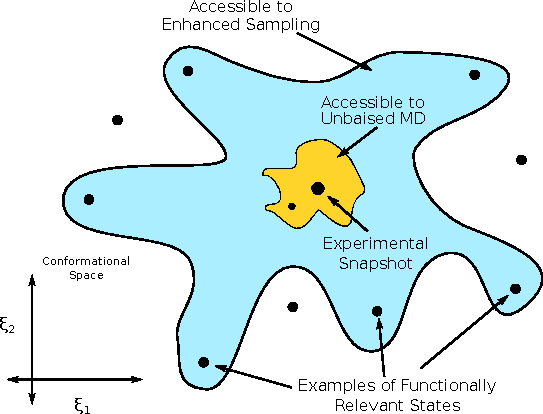
\includegraphics[width=0.6\textwidth]{figures/opening/MD_accessibility.pdf}
	\end{center}
	\captionsetup{singlelinecheck = false, justification=raggedright}
	\caption[Enhanced Sampling Allows Access to More Protein States] {\textbf{Enhanced Sampling Allows Access to More Protein States}}{The ``Resolution Revolution" in structural biolgy, fuelled by cryo-EM has lead to an era of structural abundance \cite{kuhlbrandt2014}. This means we have many structural snapshots of proteins with which to begin our study of their physical mechanisms. With unbiased MD simulations we can explore a small local neighbourhood surrounding these snapshots, shedding limited light on adjacent physilogically relevant funcational states. With Enhanced Sampling Techniques and Free energy calcuations we can access and study many more functional states. The more advanced these statistical techniques become the more functional states we will be able to access. These states might reveal drug binding pockets or the underlying mechanism behind the protein's function \cite{}. }
\end{figure}

What is perhaps remarkable about this study is just how well the results correspond with \textit{in vitro} biophysical experiments. The movements in TM1 and TM6 which dominate the PCA motions we accelerated are the kind of dilation we expected from biophysical experiments \cite{linsdell2016}. The distances from Y914 to L102 in our open state are also not much larger than those found in the cryo-EM conformation. Given that these two amino acids can be cross-linked by cysteine substitution, while still allowing the ion channel to access the open state, we would expect them to remain close together in the conducting state\cite{negoda2019}. Additionally, the similar conductance profiles between bicarbonate and chloride are are the kind we would expect from a weakly selective anion channel like CFTR \cite{}. Recall that the diffusion coefficeint of a particle scales inversely with its radius \cite{}. Since chloride is smaller than bicarbonate we would expect it to permeate more slowly through the channel, even if it passed over the same energy landscape. 4x the current, we would expect them to have a similar diffusion profile through the open channel. Indeed, the selectivity filter still ahs a constriciton of X $\AA$, so partial dehydrtaion must take place during anion conductance, so this conformation is also consistent with the lyotropic selectivity trend found in other anion channels and experimental studies of CFTR. 

We should addresse the considerable differnece in height between the  free energy minimmum which corresponds to the cryo-EM structure and the one we assert corresponds to a dilated structure. The dilated structure has a height of 17 kcal/mol compared to the lowest point in the calculated FES. At first this would seem unphysically high, indicating that the dilated state is physicaslly inaccesssible. However, there are 3 factors which we attribute to this. 

The first and most obvious is the choice of collective variables. The PCA motions outlined in Figure \ref{summary_FES} are likely suboptimal. Note for exampel how in the dilated structure in Figure \ref{summary_FES} TM1 has moved signigicanly but this motion is poorly captured by the . This motion is likely along a hiddne CV  not captured by PC1 and 2. It is interactions like this which havel ikely lead to some hysteresis in the construction of the free energy surface in Figure \ref{summary_FES}A. In future we plan to employ more advanced dimensionallity reduction techniques such as TICA and RAVE \cite{} to make a more careful choice of CVs. It is likely that the reweighting scheme of OPES-MetaD will be of great help in making these choices in future \cite{}. 

The second factor missing factor from this FES is another orthogonal degree of freedom, not captured by our collective variables. The permeation pathway through CFTR is unusually long, which means that multiple ions are likely to occupy it at any one time \cite{}. This ions are likely to have a considerable contribution to the free energy landscape calculated in Figure \ref{summary_FES}. However, .

Finally, we consider the system composition for our simulation. There is an emerging interest in the role played by the composition of the lipid bilayer in the regulation of CFTR and other annion channels. This is not due to their chemical properties, but rather their physical properties iwth differnet compositions exhibiting different lateral pressures and diffusion speeds. Hence, it is possible that the POPC membrane used here slowed the transition of walkers between the two metastable states, again leading to some levels of hysteresis in the FES. We regard the above points as room for improvement and they will be considered carefully in further studies of this dilated structure. The agreement of this structure with available biophysical evidence leads us to believe that the dilated conformation we have discovered indeed exists and further simulations will be undertaken to more carefully investigate the conduction mechanism of CFTR. 

Surprisingly, the R334W mutation was determined not to alter the relative selectivity between anions in CFTR \cite{sheppard1993}. This is an argument for a wider open pore at the R334 position, consistent with the findings of this study.

Mutagenesis studies of the R334 amino acid noticed that many different mutations appear to result in ephys readings which would indicate a loss of function, including mutation to lysine (K) which seems surprising \cite{ge2004, gong2004, linsdell2021}. One of the more common disease causing missense mutations is R334W. This motivated the use of umbrella sampling to test the energy landscape of the chloride permeation pathway in the presence of this mutation. 

We should take note of some features which are lacking from our propsed open state which we expect of the fully open structure. Careful biophysical experiments discovered an interaction between the R117 and the carboxyl atom of E1124. This interaction was not present in our open state, nor was it well preserved in our unbaised simulations of the cryo-EM conformation. Similarly, the well characterised R104-E116 interaction is poorly preserved in both simulations. In our simulations we observed that these salt bridges were often broken (in the opened and unopened states) due to interactions with phosphate head groups in the phospholipid bilayer. Given the importance of different lipid species to regulation of CFTR such as cholesterol and sphingolipids, we expect that the zwitterionic POPC lipids used as a model membrane in this study do not fully reflect the native lipid environment of CFTR \cite{farinha2018, cottrill2020}. Recent studies have demonstrated an increasing need to study the bidirectional relationship between membrane composition and membrane protein regulation \cite{lin2022, kapoor2021, cui2020}. There are sadly few examples where membrane proteins have been characterised in both in both detergents and detergent micelles and nano discs revealed different side-chain conformations (however, the backbone was conserved) \cite{autzen2019, gao2016, cheng2015}. Hence, the state of the literature suggests that the salt bridges we mentioned earlier may in fact be regulated by the local environment of lipids around those specific sections of CFTR. Readers are encouraged to undertake studies to investigate the molecular fingerprint of the environment around CFTR.

The dilated structure we present has a significant motion in TM1 . This is the kind of change we would expect from experiments studying the binding of WNK1. These studies demonstrate binding to TM1 favors the wide open conformation for the movement of bicarbonate ions \cite{kim2019}. 

As shown by the results in the present study, the difficulty in converging a free energy landscape with collective variables derived \textit {ab initio} from long classical MD simulations can be difficult as the CVs are very likely going to be suboptimal. Machine learning techniques, more sophisticated than the simple PCA algorithm used here would likely do a much better job of choosing quickly converging CVs \cite{}. 

The conformational changes investigated in this study occur within the lipid bilayer. This means that the kinetics and energetics of the transitions we have discovered will be highly dependent on the composition of lipids of the epithelium. It is well understood that the bilayer composition plays an important role in CFTR regulation and the clinical implications of this are an active area of research \cite{cui2020, cottrill2020}. It would therefore be an interesting study to repeat similar free energy calculations with different bilayer compositions to understand how they might regulate such conformational changes.

Understanding the open structure of CFTR has important implications for the drug discovery efforts to treat Cystic Fibrosis and sheds light on other important clinical questions. Specificlaly, selectivity of bicarbonate has been found to play an important role in pancreatic sufficiency of patients. The elucidation of basic CFTR function using simulations heralds an exciting new era of Cystic Fibrosis research. We are performing molecular medicine with atomic precision. 

The predictions of a stable salt bridge in section \ref{salt_bridge} fill a recent gap in the literature. The elegant study on the R117H mutation from Simon and Csnady's group \cite{simon2021}  discovered that a long standing conclusion that R117 made a connection with E1126 was incorrect and in fact R117 makes a stable hydrogen bond with E1124. This study did not closely investigate the role of E1126, observing that the E1126P mutant had slower closing kinetics but was unable to definitely explain why, suggesting that ECL6 might move slower in this mutation. This leaves the partner of E1126 unknown. One study investigating the blockage of CFTR by zinc postulated at an interaction between R334 and E1126 \cite{wang2016}. Here, the researchers tested the inhibition of chloride conduction in the presence of zinc in R334C-CFTR. They found strong evidence that R334C-CFTR was blocked by Zinc ions, as no current was recorded in the presence of zinc. Because zinc has a +2 charge they suspected that a nearby negative amino acid might might play a role in binding the zinc cation. Subsequent experiments They found that the mutant R334C/E1126A-CFTR was no longer inhibited by zinc ions. This is consistent with our findings that R334 and E1126 may indeed form a salt bridge, coming closer together in the conducting conformation compared to how far they are in the cryoEM structure.  

Previously it would have been very difficult to discover this interaction experimentally because R334 has plays such an important role in the conductance and selectivity of the channel. With the use of the atomic resolution offered by MD simulations we have been able to fill this gap in the experimental literature, demonstrating the power of \textit {in silico} methods for studying protein dynamics. We propose that single ion channel patch clamp experiments could demonstrate teh importance of teh E1126-R334 salt bridge to the open state of the channel. 

Similar to how this study was motivated by the lack of a structural picture of CFTR's conducting state, there are many other places in the proteome which would likely be amenable to a similar mode of investigation. For example, the important ABC transporter P-glycoprotein has been resolved in an outward facing occluded state, but the important outward facing conformation remains unimaged \cite{}. A similar technique to the one used here could likely resolve such a conformation \cite{kim2018a}.

\textit {in vitro} studies of the state dependent formation of the extracellular helices of the distances between  TM1, TM6, and TM12 indicated that in the closed state these helices are tightly bound together (as can be seen in the 6MSM structure) and in the open state they move apart \cite{negoda2018}. Additionally, similar studies of TM8 demonstrate that Y914 and Y917 are solvent exposed, pore lining helices, position 914 linked to position 102 and 334 when they were each replaced by cysteines. Interestingly, the distance in our proposed open structure is similar to that found in 6MSM, consistent with these experiments \cite{negoda2019}. 

Mutations at R334 also exhibit a gating defect, with infrequent transitions to the fully open state \cite{zhang2005a ,cui2013a, sheppard1993}. However, the specifics of the burst kinetics of this mutation are understudied, likely because of the low counductiviyt of the R334W-CFTR channel which makes electrophysiology experiments difficult. This reveals the niche for simuations, since we have atomic resolution into the dynamics of this channel, we can study the interacitons in the mutant where it might be hard to do experimentally. It is likely that an involved path Metadynamics or string method with swarms of trajectories approach might reveal the pathogenic gating defect present in this mutation. Construction of such a protocol could be used to investigate outher outer viestibutle gating class defects such as R117.

The simulations results we have found here would make us strongly expect a gating phenotype for an E1126 mutant to look like the R334C measuremnts found in \ref{zhang2005a}. This single ion channel study found infrequent transitions to the fully open state with frequent transitions to the transiently open state. This is consistent with the model we have proposed from our study here.

The work in this chapter suggests that computaitonal methods are now sufficiently developed such that creative application of MD simluations and free energy techniques can sehd light on the molecular mechanism of proteins. A limited but powerful example of this would be to further refine the methods applied in this chapter and then apply them to the partially collapsed structure of P-glycoprotein and dilate it in order to resolve the fully outward facing configuration.

\section{Conclusion}
With innovative application of free energy techniques we have been able to study an open, conducting conformation of CFTR. The conducting state of the channel has critical importance to drug discovery efforts for potentiators. If a small molecule drug could be developed to favor this state it would be a highly effective drug, as potentiators have demonstrated life changing clinical efficacy.

\section{Methods Details}
\subsection{System Composition}
At a basic level, methodology used in this chapter is largely consistent with the other studies in this thesis with some key differnces. The system was also constructed by embedding the extended CFTR model into a POPC membrane and then the whole these biomolecules were immersed in a neutralising 0.15 mol/L KCl solution. For all calculations in this chapter, except the initial unbiased calculations, the C-terminus was trunked at amino acid 1450 in order to make the simluation box smaller and save computer time.

\subsection{Unbiased MD }
The minimisation and equilibration steps for these simulations were largely carried out in the same way as for previous chapters. Our protein model was the extended CFTR model based on the 6MSM structure \cite{zhang2018} which we constructed in chapter \ref{chap:I37R}. The MD system was subjected to minimisation by steepest descent followed by restrained relaxation. This involved 10 kcal/mol $\AA^2$ harmonic restraints on all heavy protein atoms with restraints halved every 400 picoseconds. This relaxation was followed by up to 2.2 $\mu$s of unbiased molecular dynamics sampling.

\subsection {Principal Component and Choice of Collective Variable for OPES-Metadynamics}
Using principal component analysis on proteins can be difficult. PCA specialises in choosing the vectors which capture the \textit{largest} variation in a dataset. By contrast, when we are performing free nergy calculations we would wish to capture the \textit{slowest} motions to accelerate. This is so we can quickly converge the free energy surface along our collective variables, by choosing the slowest degrees of freedom, faster, orthogonal degrees of freedom can average out. 

So, when performing PCA on proteins, without excluding them, the motion of large, disordered loops would dominate the analysis. Hence, we limited our analysis to the amino acids in the transmembrane helices in Table \ref{red_alpha_carbons_table}. 

For the sake of performance, a smaller subset of amino acids were then chosen to actually manipulate the proe of CFTR in the OPES-Metadynamics simulations. These calculations were expensive and the more atoms included in our CVs the slower the calculations were run, so the amino acids highlighted in red in Table \ref{red_alpha_carbons_table} were chosen for furhter analysis. These were the pore lining amino acids and our choses closely reflect those of previous studies (Figure \ref{pore_lining_PCA}) \cite{hoffman2018}. 

\begin{table}
	\begin{center}
	%\begin{tabular} {| c | c | c | c | c | c | c | c | c | c | c | c | }  
	\resizebox{0.85\textwidth}{!}{%
	\begin{tabular} {| c | c | c | c | c | c | c | c | c | c | c | c | }  
		\hline
		\textbf{TM1}  $\uparrow$ & \textbf{TM2}  $\downarrow$ & \textbf{TM3}  $\uparrow$ & \textbf{TM4}   $\downarrow$& \textbf{TM5}  $\uparrow$ & \textbf{TM6}   $\downarrow$& \textbf{TM7}  $\uparrow$ & \textbf{TM8}   $\downarrow$& \textbf{TM9}   $\uparrow$& \textbf{TM10} $\downarrow$ & \textbf{TM11}  $\uparrow$ & \textbf{TM12}   $\downarrow$\\ \hline

                         & 113                      &  218 & 219 &                          &                          & 885 &                          &                           & 1013 &                            &                           \\ \hline
                         & 114                      &  217 & 220 &                          &                          & 884 &                          &                           & 1014 &                            &                           \\ \hline
                         & 115                      &  216 & 221 &                          &                          & 883 &                          &                           & 1015 &                            &                           \\ \hline
                         & 116                      &  215 & 222 &                          &                          & 882 &                          &                           & 1016 &                            &                           \\ \hline
                         & 117                      &  214 & 223 &                          &                          & 881 &                          &                           & 1017 &                            &                           \\ \hline
112                      & 118                      &  213 & 224 & 330                      &                          & 880 &                          &                           & 1018 &                            & 1124                      \\ \hline
111                      & 119                      &  212 & 225 & 329                      & 331                      & 879 & 911                      &                           & 1019 &                            & 1125                      \\ \hline
110                      & 120                      &  211 & 226 & 328                      & 332                      & 878 & 912                      & 1012                      & 1020 & 1123                       & 1126                      \\ \hline
109                      & 121                      &  210 & 227 & 327                      & 333                      & 877 & 913                      & 1011                      & 1021 & 1122                       & 1127                      \\ \hline
\cellcolor{red!25}108 & \cellcolor{red!25}122 &  209 & 228 & \cellcolor{red!25}326 & \cellcolor{red!25}334 & 876 & \cellcolor{red!25}914 & \cellcolor{red!25}1010 & 1022 & \cellcolor{red!25}1121  & \cellcolor{red!25}1128 \\ \hline
\cellcolor{red!25}107 & \cellcolor{red!25}123 &  208 & 229 & \cellcolor{red!25}325 & \cellcolor{red!25}335 & 875 & \cellcolor{red!25}915 & \cellcolor{red!25}1009 & 1023 & \cellcolor{red!25}1120  & \cellcolor{red!25}1129 \\ \hline
\cellcolor{red!25}106 & \cellcolor{red!25}124 &  207 & 230 & \cellcolor{red!25}324 & \cellcolor{red!25}336 & 874 & \cellcolor{red!25}916 & \cellcolor{red!25}1008 & 1024 & \cellcolor{red!25}1119  & \cellcolor{red!25}1130 \\ \hline
\cellcolor{red!25}105 & \cellcolor{red!25}125 &  206 & 231 & \cellcolor{red!25}323 & \cellcolor{red!25}337 & 873 & \cellcolor{red!25}917 & \cellcolor{red!25}1007 & 1025 & \cellcolor{red!25}1118  & \cellcolor{red!25}1131 \\ \hline
\cellcolor{red!25}104 & \cellcolor{red!25}126 &  205 & 232 & \cellcolor{red!25}322 & \cellcolor{red!25}338 & 872 & \cellcolor{red!25}918 & \cellcolor{red!25}1006 & 1026 & \cellcolor{red!25}1117  & \cellcolor{red!25}1132 \\ \hline
\cellcolor{red!25}103 & \cellcolor{red!25}127 &  204 & 233 & \cellcolor{red!25}321 & \cellcolor{red!25}339 & 871 & \cellcolor{red!25}919 & \cellcolor{red!25}1005 & 1027 & \cellcolor{red!25}1116  & \cellcolor{red!25}1133 \\ \hline
\cellcolor{red!25}102 & \cellcolor{red!25}128 &  203 & 234 & \cellcolor{red!25}320 & \cellcolor{red!25}340 & 870 & \cellcolor{red!25}920 & \cellcolor{red!25}1004 & 1028 & \cellcolor{red!25}1115  & \cellcolor{red!25}1134 \\ \hline
\cellcolor{red!25}101 & \cellcolor{red!25}129 &  202 & 235 & \cellcolor{red!25}319 & \cellcolor{red!25}341 & 869 & \cellcolor{red!25}921 & \cellcolor{red!25}1003 & 1029 & \cellcolor{red!25}1114  & \cellcolor{red!25}1135 \\ \hline
\cellcolor{red!25}100 & 130                      &  201 & 236 & \cellcolor{red!25}318 & \cellcolor{red!25}342 & 868 & \cellcolor{red!25}922 & 1002                      & 1030 & 1113                       & \cellcolor{red!25}1136 \\ \hline
\cellcolor{red!25} 99 & 131                      &  200 & 237 & 317                      & 343                      & 867 & 923                      & 1001                      & 1031 & 1112                       & \cellcolor{red!25}1137 \\ \hline
 98                      & 132                      &  199 & 238 & 316                      & 344                      & 866 & 924                      & 1000                      & 1032 & 1111                       & \cellcolor{red!25}1138 \\ \hline
 97                      & 133                      &  198 & 239 & 315                      & 345                      & 865 & 925                      &  999                      & 1033 & 1110                       & 1139                      \\ \hline
 96                      & 134                      &  197 & 240 & 314                      & 346                      & 864 & 926                      &  998                      & 1034 & 1109                       & 1140                      \\ \hline
 95                      & 135                      &  196 & 241 & 313                      & 347                      & 863 & 927                      &  997                      & 1035 & 1108                       & 1141                      \\ \hline
 94                      & 136                      &  195 & 242 & 312                      & 348                      & 862 & 928                      &  996                      & 1036 & 1107                       & 1142                      \\ \hline
 93                      & 137                      &  194 & 243 & 311                      & 349                      & 861 & 929                      &  995                      & 1037 & 1106                       & 1143                      \\ \hline
 92                      & 138                      &  193 & 244 & 310                      & 350                      & 860 & 930                      &  994                      & 1038 & 1105                       & 1144                      \\ \hline
 91                      & 139                      &  192 & 245 & 309                      & 351                      & 859 & 931                      &  993                      & 1039 & 1104                       & 1145                      \\ \hline
 90                      & 140                      &  191 & 246 & 308                      & 352                      & 858 & 932                      &  992                      & 1040 & 1103                       & 1146                      \\ \hline
 89                      & 141                      &  190 & 247 & 307                      & 353                      & 857 & 933                      &  991                      & 1041 & 1102                       & 1147                      \\ \hline
 88                      & 142                      &  189 & 248 & 306                      & 354                      & 856 & 934                      &  990                      & 1042 & 1101                       & 1148                      \\ \hline
 87                      & 143                      &  188 & 249 & 305                      & 355                      & 855 & 935                      &  989                      & 1043 & 1100                       & 1149                      \\ \hline
 86                      & 144                      &  187 & 250 & 304                      & 356                      & 854 & 936                      &  988                      & 1044 & 1099                       & 1150                      \\ \hline
 85                      & 145                      &  186 & 251 & 303                      & 357                      & 853 & 937                      &  987                      & 1045 & 1098                       & 1151                      \\ \hline
 84                      & 146                      &  185 & 252 & 302                      & 358                      & 852 & 938                      &  986                      & 1046 & 1097                       & 1152                      \\ \hline
 83                      & 147                      &  184 & 253 & 301                      & 359                      & 851 & 939                      &  985                      & 1047 & 1096                       & 1153                      \\ \hline
 82                      & 148                      &  183 & 254 & 300                      & 360                      & 850 & 940                      &  984                      & 1048 & 1095                       & 1154                      \\ \hline
 81                      & 149                      &  182 & 255 & 299                      & 361                      & 849 & 941                      &  983                      & 1049 & 1094                       & 1155                      \\ \hline
 80                      & 150                      &  181 & 256 & 298                      & 362                      & 848 & 942                      &  982                      & 1050 & 1093                       & 1156                      \\ \hline
 79                      & 151                      &  180 & 257 & 297                      & 363                      & 847 & 943                      &  981                      & 1051 & 1092                       & 1157                      \\ \hline
 78                      & 152                      &  179 & 258 & 296                      & 364                      & 846 & 944                      &  980                      & 1052 & 1091                       & 1158                      \\ \hline
 77                      & 153                      &  178 & 259 & 295                      & 365                      & 845 & 945                      &  979                      & 1053 & 1090                       & 1159                      \\ \hline
 76                      & 154                      &  177 & 260 & 294                      & 366                      & 844 & 946                      &  978                      & 1054 & 1089                       & 1160                      \\ \hline
 75                      & 155                      &  176 & 261 & 293                      & 367                      &     & 947                      &  977                      & 1055 & 1088                       & 1161                      \\ \hline
 74                      & 156                      &  175 & 262 & 292                      & 368                      &     & 948                      &  976                      & 1056 & 1087                       & 1162                      \\ \hline
 73                      & 157                      &  174 & 263 & 291                      & 369                      &     & 949                      &  975                      & 1057 & 1086                       & 1163                      \\ \hline
 72                      & 158                      &  173 & 264 & 290                      & 370                      &     & 950                      &  974                      & 1058 & 1085                       & 1164                      \\ \hline
                         & 159                      &  172 & 265 & 289                      & 371                      &     & 951                      &  973                      & 1059 & 1084                       & 1165                      \\ \hline
                         & 160                      &      & 266 & 288                      & 372                      &     & 952                      &  972                      & 1060 & 1083                       & 1166                      \\ \hline
                         & 161                      &      & 267 & 287                      & 373                      &     & 953                      &  971                      & 1061 & 1082                       & 1167                      \\ \hline
                         & 162                      &      & 268 & 286                      & 374                      &     & 954                      &  970                      & 1062 & 1081                       & 1168                      \\ \hline
                         & 163                      &      & 269 & 285                      & 375                      &     & 955                      &  969                      & 1063 & 1080                       & 1169                      \\ \hline
                         & 164                      &      & 270 & 284                      & 376                      &     & 956                      &  968                      & 1064 & 1079                       &                           \\ \hline
                         & 165                      &      & 271 & 283                      & 377                      &     & 957                      &  967                      & 1065 & 1078                       &                           \\ \hline
                         & 166                      &      & 272 & 282                      &                          &     & 958                      &  966                      & 1066 & 1077                       &                           \\ \hline
                         & 167                      &      & 273 & 281                      &                          &     & 959                      &  965                      & 1067 & 1076                       &                           \\ \hline
                         & 168                      &      &     & 280                      &                          &     & 960                      &                           &      & 1075                       &                           \\ \hline
                         & 169                      &      &     & 279                      &                          &     & 961                      &                           &      & 1074                       &                           \\ \hline
                         & 170                      &      &     & 278                      &                          &     & 962                      &                           &      & 1073                       &                           \\ \hline
                         & 171                      &      &     & 277                      &                          &     & 963                      &                           &      & 1072                       &                           \\ \hline
						 &                          &      &     & 276                      &                          &     & 964                      &                           &      & 1071                       &                           \\ \hline
						 &                          &      &     & 275                      &                          &     &                          &                           &      & 1070                       &                           \\ \hline
            			 &                          &      &     & 274                      &                          &     &                          &                           &      & 1069                       &                           \\ \hline
						 &                          &      &     &                          &                          &     &                          &                           &      & 1068                       &                           \\ \hline
 
            



\end{tabular}%
}
\end{center}
\captionsetup{singlelinecheck = false, justification=raggedright}                           
\caption[Amino acids used to analyse and manipulate the outer pore of CFTR] {\textbf{Amino acids used to analyse and manipulate the outer pore of CFTR}}{All listed amino acids were included in the unbiased extraction of PCA components. The cells highlighted in red denote the amino acids which were used as collective variables to study the free energy landscape of PCA motions 1 and 2. These are visualised in Figure \ref{steer_cas_fig}. }

\label{red_alpha_carbons_table}
\end{table}

\begin{figure}
	\begin{center}
		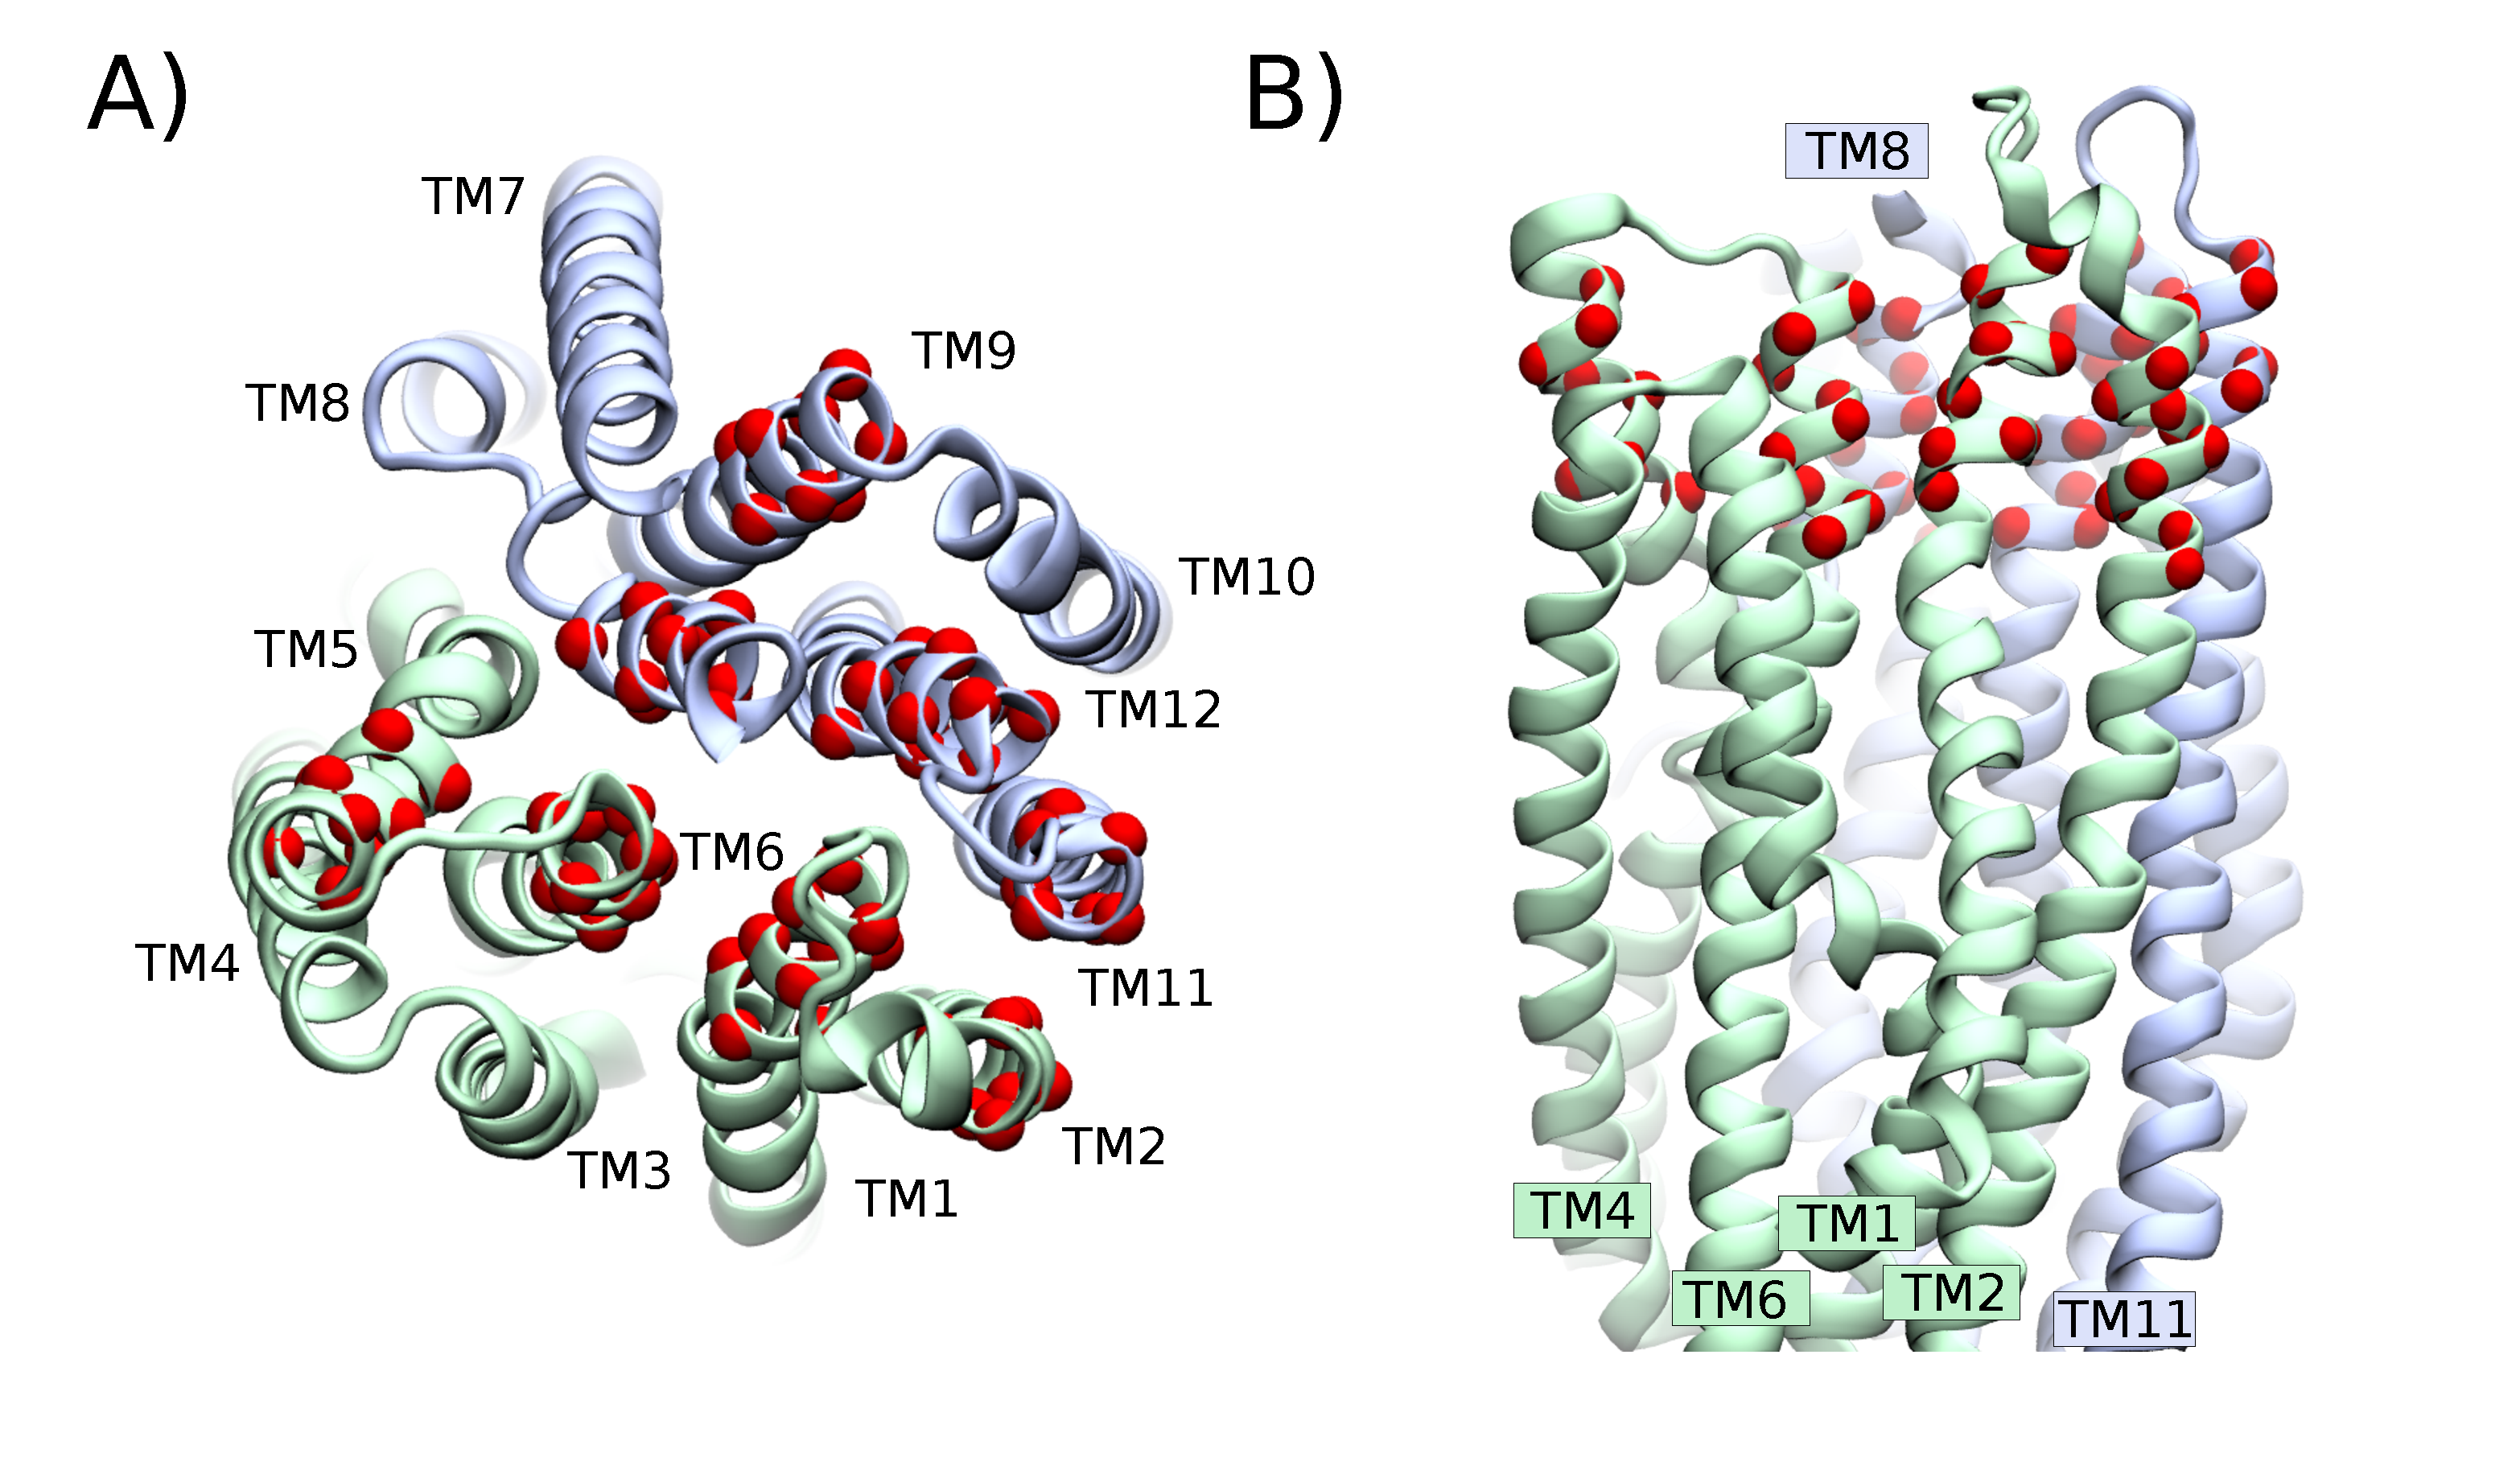
\includegraphics[width=1\textwidth]{figures/opening/steer_cas.pdf}
	\end{center}
	\captionsetup{singlelinecheck = false, justification=raggedright}
	\caption[The Alpha Carbon Atoms Manipulated to Dilate CFTR] {\textbf{The Alpha Carbons Manipulated to Dilate CFTR}}{the Alpha Carbon Atoms used to manipulate the pore of CFTR. The motion of the alpha carbon atoms, represented as red spheres, which were pushed along PC1 and 2 during OPES-MetaD calculations to study the dilation of the CFTR pore. A) A top down view, note how pore lining helices have been selected for manipulation. B) A side-on view. Note how the upper section of the selectivity filter has been selected for manipulation. These choices of amino acids were made to proritise the dilation of the extracellular mouth of the channel, which closely reflects the philosophy of previous studies \cite{hoffman2018}. } 
	\label{steer_cas_fig}
\end{figure}

%By selecting this subset, we applied Principal Component Analysis to the combined, aligned timeseries data from the alpha carbons of the amino acids in table \ref{pca_aas}. This allowed our analysis to focus on the slow, large motions which would most likely dilate the channel. The first 9 Principal Components were inspected visually. By the 4th vector, the motions were comparatively small and hence our analysis focussed on the first two motions. Motions 1 and 2 produced large movments in TM1 and TM6 which was where we expected the extracellular mouth to dilate. Hence, we chose to accelerate these first two motions.

\subsection{OPES-MetaD}
We employed 8 parralel walkers in order to properly explore and converge the free energy landscape along the two PCA motions studied in this chapter. On the Fly Probability Enhanced Sampling was used to converge this difficult free energy landscape \cite{}. Since we did not know exactly what kind of conformational change to expect and we had no \textit {ab initio} method to assess the quality of our CVs, a large barrier height of 38.2 kcal/mol was chosen for the OPES-MetaD protocol. In order to decrease computational expense, masses were redistributed throughout the system using the conventional approach to Hydrogen Mass Repartitioning. This allowed us to increase the simluation timestep to 4 femtsoconed. Gaussians were deposited every 500 simulation time steps.

Convergence was acheived after  Figure \ref{convervengfece_fig} revleas how inspection of the constructed free energy surface at 100ns time intervals demonstrates a converged free energy surface. Convergence was achieved after  was 1.5 $\mu$s of sampling for each walker, for a total of 12 microseconds of sampling.

This is confirmed by further inspection of OPES-MetaD vairables in figure \ref{Z_sigma_fig}. The $Z$ parameter from OPES-MetaD which measures the amount of new CV space explored by the simulation. Convergence implies that hte whole accessible volume at a given barrier parmater has been sampled. Similarly, convergence of the $c(t) = \frac{1}{\beta} \log \langle e^{\beta V} \rangle$ parameter in figure \ref{Z_sigma_fig}B indicates the free energy surface has stopped evolving. 

\subsection{Umbrella Sampling}
All Umbrella sampling studies were carried out with the same methodology. In the unbiased equilibration steps of a CFTR simulation, an anion was found to occupy the inner vestibule. 

The collective variable in each simulation was constructed by calculating the z coordinate of the center of mass of the alpha carbon atoms from the amino acids in table \ref{red_alpha_carbons} and then subtracting the z position of the steered anion. The radial position of the ion was restrained a half potential well, when the ion strayed more than 4.8 $\AA$ from the center axis of the CFTR channel it would encounter a repulsive 10kcal/mol $\AA^2$ harmonic potential. This meant the ion could not stray too far from the center axis when it simulated in the bulk region but did mean that the ion could adequately sample the interior of the selectivity filter.

In order to calculate the PMF through the channel, we steered this annion to the middle of the channel over the course of 10ns and allowed it to equilibrate there for 20 ns. The annion was then steered to its target location over the course of 10ns depending on which window that particular simulation belonged to. It was then restrained at this location for the 50ns production run.

To calculation the PMF along of the anion through the selectivity filter we collected the distance Z every picoseconds for 50ns. This data was then binned into 5 independent blocks of 10 nanoseconds and an individual PMF was constructed suing hte Weighted Histrograms Analysis Method (WHAM). The independent PMF profiles were then aligned at their extreme end (42-48 $\AA$) which correspondents to the flat energy surface  obtained from pulling pulling a chloride ion through bulk solvent. The Uncertainties were then caluclated by claculating the Standard Error of the Mean between tehse 5 independent samples with this alignment technique. Similarly, comparisons between the PMFS from different CFTR systems were also constructed by using the region of the PMF which corresponds to  bulk solvent (42-48 $\AA$) as an aboslute reference point.
